\clearpage

\section{Systematic effects in the prediction of the single $\mu$-like ring and single e-like ring event reconstructed energy spectra in SuperK}
%\section{Updated systematic effects in the prediction of the single $\mu$-like ring and single e-like ring event reconstructed energy spectrum}
\label{sec:systematics}

There are 64 systematic parameters considered in this analysis. 
They will be described now, grouped into 4 categories:

\begin{enumerate}

%%%% ENERGY SCALE 

\item 
{\bf SuperK energy scale} (1 parameter).\\
The systematic parameter $f_{E; r}^{SK}$ is included to account for the energy scale uncertainty, 
which is estimated to be 2.4\% \cite{SuperkEScale2013}.
This systematic parameter is applied differently to the other systematics, since it is not applied as a weight in the number of events in each bin. 
The effect of the uncertainty in the reconstructed energy scale is computed by scaling the bin edges of
the MC templates and, assuming uniform distribution of events within the bins, calculating the number
of events gained from / lost to neighbouring bins. 
The effect of the energy scale uncertainty is propagated to all MC templates as shown in Tab.\ \ref{tab:apply_syst_to_1Rmu_templates} and \ref{tab:apply_syst_to_1Re_templates}.\\


%%%% SK + FSI + SI 

\item 
{\bf SuperK efficiencies \& effects of intranuclear and secondary re-interactions \& Photo nuclear effects } (6+12 parameters).\\

There are uncertainties in the efficiencies of the cuts used to select single ring events at SuperK: the fiducial volume and reduction chain, and the OD, ring-counting, PID, momentum and decay-electron cuts.
These uncertainties are evaluated comparing SK-IV atmospheric data with atmospheric neutrino Monte Carlo.
For the 2013 joint oscillation analysis, these uncertainties were evaluated taking into account correlations between
the two single $\mu$-like ring and single e-like ring event samples \cite{SKcorrelations}.
Very pure samples of atmospheric neutrinos with either single $\mu$-like ring or single e-like ring events at the final state were selected. Those samples are fitted to the data including constraints from control samples (stopping cosmic muons and hybrid $\pi^0$ samples), using a Markov-Chain Monte Carlo method with the efficiencies as fit parameters (see details in \cite{PatrickPlenary}).
Finally, the covariance matrix is calculated using toy MC experiments as explained in \cite{ImberTalk}. 

Intranuclear final-state interactions (FSI) have significant effects in the T2K energy range and
result in event topologies, for scattering from nuclear targets, which are drastically different from 
those created in neutrino scattering from free nucleons.
Uncertainties due to FSI were estimated by simultaneously varying the NEUT parameters that scale the interaction probabilities for quasi-elastic 
scattering, absorption, charge exchange and pion production using the method described in Sec.\ 2 in \cite{NIWGErr}. 
Uncertainties due to secondary pion interactions (SI) were also evaluated. Since the same model is used for FSI and SI, it is possible to evaluate the uncertainties in both FSI and SI simultaneously. 
For each stand-alone analysis, $\nu_{\mu}$ disappearance or $\nu_{e}$ appearance analysis, the same set of 8 FS+SI  parameters is used. 
The effect of FSI+SI uncertainties is estimated by reweighting at the same time single $\mu$-like ring and single e-like selected SK MC events 
with the same 8 parameters set for both samples using T2KReweight, and finding the number of events in each one of the 18 event categories 
(6 categories in $\nu_{\mu}$ disappearance and 12 categories $\nu_{e}$ appearance, the same as the final parametrization of SK+FSI+SI parameters).
The reweighting method for FSI is described in Sec. 8 in \cite{NEUTnuclear}. Variations in the SI interaction probabilities were included for each FSI parameter set. 
Subsequently a covariance matrix was calculated using equation 1 in \cite{NIWGErr}; the quantity p in that equation is the average event weight for a FSI parameter set, and 
the sum is over the parameter sets. This covariance matrix contains correlations between the two single $\mu$-like ring and single e-like ring events samples \cite{ikeda}.

For this analysis, systematic errors related to Photo Nuclear effects (interactions between photons and nuclei) were taken into account following the work done for the stand-alone appearance analyses. The identification of a $\pi^0$ relies on the detection of the two photons produced by this particle, but a photon can be absorbed before emitting Cerenkov light, being therefore undetected, and this would create an additional uncertainty for the interaction modes where a $\pi^0$ is produced. 
A covariance matrix has been calculated for the PN uncertainty using the fiTQun $\pi^0$ cut, in the same binning used for the stand-alone appearance analysis SK and FSI systematic errors \cite{2013nueptheta}, \cite{2013nuenergy}.

In this analysis,the SuperK detector efficiency and FSI+SI systematics are considered together, adding their covariance matrices linearly, what it is possible since the same binning is used for both covariance matrices. Then, the PN covariance matrix is added linearly to the SK+FSI submatrix (12 x 12) related to the single e-like ring sample. Details of these uncertainties are given in 
Tab.\ \ref{tab:input_uncertainties}, and the final SK+FSI+SI+PN covariance matrix and fractional errors are presented in \ref{eq:Cskfsi} and \ref{fig:skfsi_frac} respectively. These efficiency/FSI/SI systematics are applied to the MC templates as shown in Tab.\ \ref{tab:apply_syst_to_1Rmu_templates} and \ref{tab:apply_syst_to_1Re_templates}.\\

%%%%% BANFF

\item 
{\bf Correlated flux and cross-section (BANFF) parameters} (33 parameters).\\

The postfit uncertainties of all BANFF flux and cross-section parameters and their correlations are taken into account.
The version of the BANFF fit is slightly different for the stand-alone disappearance, stand-alone appearance and joint oscillation analyses. 
Concerning the flux parameters, for the stand-alone disappearance analysis the version of the BANFF fit considers only the $\nu_\mu$ and $\bar{\nu}_{\mu}$ flux parameters, whereas for the stand-alone appearance flux parameters are considered for $\nu_\mu$, $\bar{\nu}_{\mu}$, $\nu_e$ and $\bar{\nu}_{e}$, with a smaller number of $\bar{\nu}_{\mu}$ flux bins than the stand-alone disappearance analysis. The BANFF version for the joint analysis includes flux bins for $\nu_\mu$, $\bar{\nu}_{\mu}$, $\nu_e$ and $\bar{\nu}_{e}$, with the number of flux bins for $\bar{\nu}_{\mu}$ from the stand-alone disappearance analysis. 
There are also differences in the number of correlated cross-section parameters included in the different BANFF versions for the stand-alone analyses and the joint analysis. For the stand-alone disappearance analysis, there are three CCQE normalization parameters (0-1.5 GeV, 1.5-3.5 GeV and 3.5-30 GeV) and two for the CC1$\pi$ normalization (1.5-3.5 GeV and 3.5-30 GeV), whereas for the stand-alone appearance analysis only one parameter is consider for each normalization, the one in the lower energy range. There is also one extra parameter in the stand-alone appearance analysis with respect to the stand-alone disappearance analysis: this is the NC1$\pi^{0}$ normalization parameter. The BANFF version produced for the joint analysis considers all the cross-section parameters included in the stand-alone disappearance and stand-alone appearance versions (8 in total), however, the NC1$\pi^{0}$ normalization parameter is only applied to the single e-like ring sample templates, because there are no single $\mu$-like ring NC1$\pi^{0}$ templates.

A summary of the list of parameters included in the BANFF postfit files for each oscillation analysis is given in Tab. \ref{tab:banff}

\begin{table}[h]
\centering
\begin{tabular}{|c||c|c|c|}
\hline
Parameter & $\nu_{\mu}$-disappearance analysis & $\nu_{e}$-appearance analysis  & joint analysis\\
\hline \hline
\multirow{4}{*}{$\nu_{\mu}$ flux} & 0-0.4, 0.4-0.5, 0.5-0.6, &  0-0.4, 0.4-0.5, 0.5-0.6, &   0-0.4, 0.4-0.5, 0.5-0.6,\\
 & 0.6-0.7, 0.7-1.0, 1.0-1.5, & 0.6-0.7, 0.7-1.0, 1.0-1.5, & 0.6-0.7, 0.7-1.0, 1.0-1.5, \\
 & 1.5-2.5, 2.5-3.5, 3.5-5.0,  & 1.5-2.5, 2.5-3.5, 3.5-5.0,  & 1.5-2.5, 2.5-3.5, 3.5-5.0, \\
&  5.0-7.0, 7.0-30.0 \bf{(11 bins)}  &  5.0-7.0, 7.0-30.0 \bf{(11 bins)}  &  5.0-7.0, 7.0-30.0 \bf{(11 bins)} \\
\hline
\multirow{2}{*}{$\bar{\nu_{\mu}}$ flux }& 0-0.7, 0.7-1.0, 1.0-1.5, &  0-1.5, 1.5-30.0 \bf{(2 bins)}  & 0-0.7, 0.7-1.0, 1.0-1.5,\\
& 1.5-2.5, 2.5-30.0 \bf{(5 bins)} & & 1.5-2.5, 2.5-30.0 \bf{(5 bins)}\\
\hline
\multirow{3}{*}{$\nu_{e}$ flux} & -- &  0-0.5, 0.5-0.7, 0.7-0.8, & 0-0.5, 0.5-0.7, 0.7-0.8, \\
& & 0.8-1.5, 1.5-2.5, 2.5-4.0, & 0.8-1.5, 1.5-2.5, 2.5-4.0, \\
& &  4.0-30.0 \bf{(7 bins)} &  4.0-30.0 \bf{(7 bins)} \\
\hline
$\bar{\nu_{e}}$ flux & -- & 0-2.5, 2.5-30.0 \bf{(2 bins)} & 0-2.5, 2.5-30.0 \bf{(2 bins}) \\
\hline \hline
$M_{A}^{QE}$ & \ck & \ck & \ck \\
\hline
$M_{A}^{RES}$ & \ck & \ck & \ck\\
\hline
CCQE normalization (0-1.5 GeV) & \ck & \ck & \ck\\
\hline
CCQE normalization (1.5-3.5 GeV) & \ck & -- & \ck\\
\hline
CCQE normalization (3.5-30. GeV) & \ck & -- & \ck\\
\hline
CC1$\pi$ normalization (0-2.5 GeV) & \ck & \ck & \ck\\
\hline
CC1$\pi$ normalization (2.5-30 GeV) & \ck & -- & \ck\\
\hline
NC1$\pi^{0}$ normalization & -- & \ck & \ck\\
\hline
\end{tabular}
\caption{List of parameters included in the BANFF postfit files, varying depending on the different versions produced for each oscillation analysis.}
\label{tab:banff}
\end{table}

%{tab:apply_syst_to_samples}


A list of the BANFF parameters, their best-fit values and their prefit and postfit errors is given in Tab.\ \ref{tab:input_uncertainties} and Fig. \ref{fig:banff}.

The BANFF parameters are applied to the MC templates as specified in Tab.\ \ref{tab:apply_syst_to_1Rmu_templates} and \ref{tab:apply_syst_to_1Re_templates}.
Among the BANFF cross-section parameters, all but two are simple normalization factors. 
However, the parameters $f_{25; t, r}^{banff}$ and $f_{26; t, r}^{banff}$, the ones corresponding to the 
axial masses ( CC quasi-elastic, $M_{A}^{QE}$, and resonance-production, $M_{A}^{RES}$ respectively), have a more complicated, often non-linear, dependence on true and reconstructed neutrino energy.
For this reason, event reweighting methods were used to obtain the fractional changes of the number of events
in bins of true and reconstructed neutrino energy, for a range of values (-3.0$\sigma$, -2.5$\sigma$, -2.0$\sigma$, ..., +3.0$\sigma$) for the $f_{25; t, r}^{banff}$ and $f_{26; t, r}^{banff}$ parameters.
In our p.d.f. calculation, cubic splines

\footnote{
  In this analysis, as in the \textit{VALOR} stand-alone disappearance analysis \cite{OurRun1234DisappAnalysis3Flavour},
 the cubic splines are computed for each non-linear systematic and for each MC template,
  in bins of reconstructed and true energy. To produce these splines, the SK13a SuperK MC, the 11bv3.2 flux weights are used and the following oscillation parameters: $\sin^{2}(2\theta_{23})$ = 1.0, $\sin^{2}(2\theta_{13})$ = 0.098, $\sin^{2}(2\theta_{12})$ = 0.8495, $|\Delta m^{2}_{32}|$ = 2.44$\times$10$^{-3}$ eV$^{2}$/c$^{4}$, $\Delta m^{2}_{21}$ = 7.5$\times$10$^{-5}$ eV$^{2}$/c$^{4}$, $\delta_{CP}$ = 0 and the normal mass hierarchy. 
The splines for the single $\mu$-like ring sample were made using 41 bins in reconstructed energy:
  1 bin from 0-0.3 GeV, 14 50-MeV bins from 0.3-1.0 GeV, 20 100-MeV bins from 1.0-3.0 GeV, 2 500-MeV bins from 3.0-4.0 GeV, 1 bin from 4.0-5.0 GeV, 1 bin from 5.0-7.0 GeV, 1 bin from 7.0-10.0 GeV and 1 bin from 10.0-30.0 GeV.
  The $\nu_{\mu}$, $\bar{\nu}_{\mu}$ and oscillated $\nu_{e}$ selections for the single $\mu$-like ring sample have 11 bins in true energy:
  1 bin from 0-0.4 GeV, 3 100-MeV bins from 0.4-0.7 GeV, 1 bin from 0.7-1.0 GeV, 1 bin from 1.0-1.5 GeV, 2 1-GeV bins from 1.5-3.5 GeV,  1 bin from 3.5-5.0 GeV, 1 bin from 5.0-7.0 GeV and 1 bin from 7.0-30.0 GeV, 
and the $\nu_{e}$ and oscillated $\nu_\mu$ samples have 7 bins in true energy:
  1 bin from 0-0.05 GeV, 1 bin from 0.5-0.7 GeV, 1 bin from 0.7-0.8 GeV,
  1 bin from 0.8-1.5 GeV, 1 bin from 1.5-2.5 GeV, 1 bin from 2.5-4.0 GeV and 1 bin from 4.0-30.0 GeV,
  and finally, the $\bar{\nu}_{e}$ sample have 2 bins in true energy:
  1 bin from 0-2.5 GeV and 1 bin from 2.5-30.0 GeV. The binning of the cubic splines for the single $\mu$-like ring events was studied, and the results were presented in Appendix I of \cite{OurRun123DisappAnalysis3Flavour}. \\
For the single e-like ring sample splines the reconstructed and true energy bins used were the same ones used for the
stand-alone appearance analyses. Therefore, reconstructed energy bins of 50 MeV were used from 0-1.25 GeV for $\nu_{\mu}$, $\bar{\nu}_{\mu}$,$\nu_{e}$, $\bar{\nu}_{e}$ and oscillated $\nu_{e}$. The binning for true energy for the single e-like ring events coincide with the one used for the single $\mu$-like ring events, with the exception of the oscillated $\nu_{e}$ sample, which uses in the single e-like ring sample the following 7 bins in true energy:
  1 bin from 0-0.05 GeV, 1 bin from 0.5-0.7 GeV, 1 bin from 0.7-0.8 GeV,
  1 bin from 0.8-1.5 GeV, 1 bin from 1.5-2.5 GeV, 1 bin from 2.5-4.0 GeV and 1 bin from 4.0-30.0 GeV.
  The spline spectra produced using the cubic splines are very similar to those produced using the CPU-intensive event-by-event reweighting, especially for the dominant components of the spectra. 
} are used to interpolate between these event weights 
to obtain the fractional change for any value of these systematic parameters in the (-3.0$\sigma$, +3.0$\sigma$) range.
An example of one cubic spline is presented in Fig. \ref{fig:spline}.\\

%% SPLINE EXAMPLE PLOT
\begin{figure*}[htb]
\center
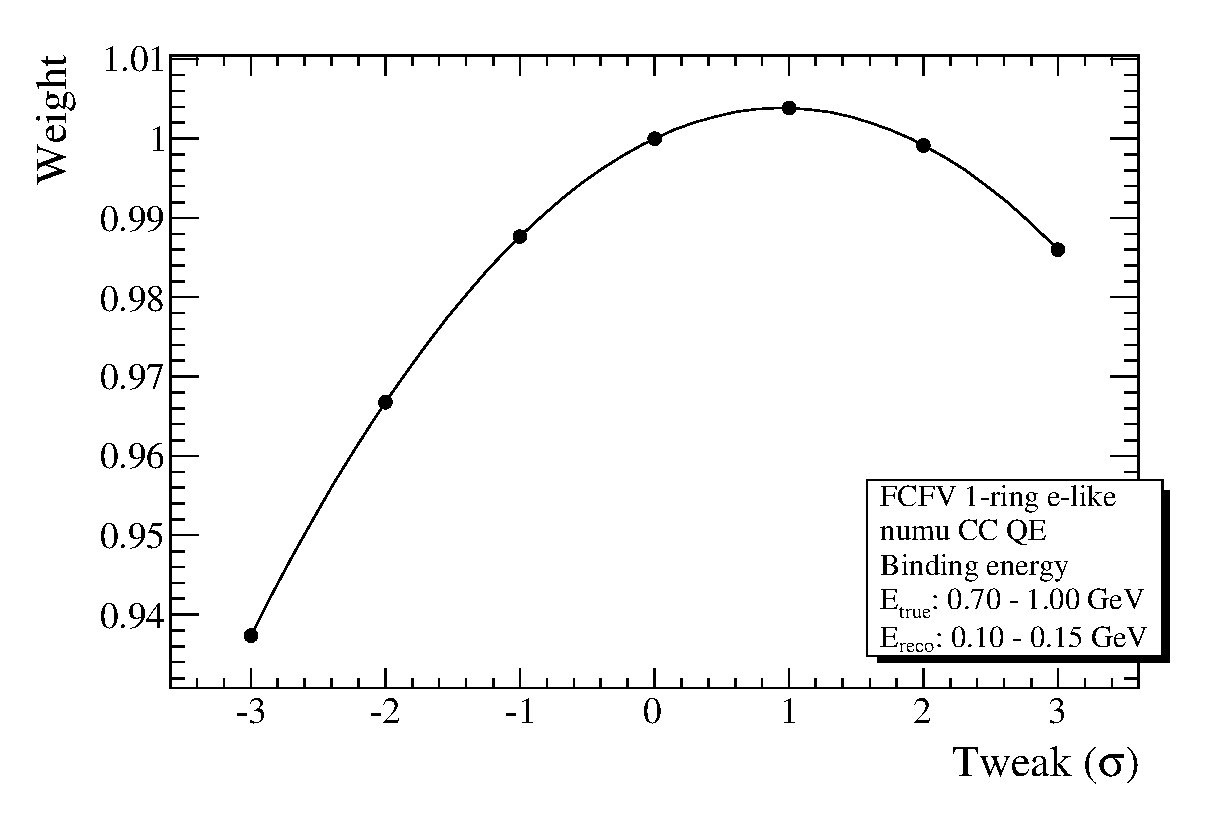
\includegraphics[width=30pc]{./images/systematics/spl_1Re_numuccqe_f_bindE_3_4.eps}
\caption {
  Example of response function (cubic spline) showing the weight vs the tweak for the Binding Energy systematic parameter
for the 1R$_e$ sample, $\nu_{\mu}$ CCQE interaction mode, $E_{true}$ between 0.7-1.0 GeV and $E_{reco}$ between 0.10-0.15 GeV.
}
\label{fig:spline}
\end{figure*}



%%% UNCORRELATED CROSS SECTIONS

\item 
{\bf Uncorrelated cross-section parameters}(12 parameters).\\

In addition to the BANFF cross-section systematics,
another 12 cross-section systematics are taken into account; these additional systematics are considered to be uncorrelated 
between themselves and to have no cancellation between the near and far detectors \cite{NIWGErr} \cite{MoreNIWGErr113} \cite{NIWGNuBarErr}.

There are some differences in the list of uncorrelated cross-section parameters between the different oscillation analyses. 
There is one systematic parameter which is only consider in the stand-alone appearance analysis, but not in the stand-alone disappearance analysis: this is the NC coherent cross-section parameter. On the other hand, there are three cross-section systematics that are used in the stand-alone disappearance analysis but not in the stand-alone appearance analysis: the systematic for the Binding Energy, the NC1$\pi^{\pm}$ cross-section and the $\sigma_{\bar{\nu}}/\sigma_{\nu}$ ratio. The joint oscillation analysis considers them all (12 parameters) although the NC coherent cross-section parameter is only applied to the single e-like ring NC coherent templates (there are no single $\mu$-like ring NC coherent templates) and the  NC1$\pi^{\pm}$ cross-section parameter is only applied to the single $\mu$-like ring NC1$\pi^{\pm}$ templates (there are no single e-like ring NC1$\pi^{\pm}$ templates).

Three of these additional systematics relate to the initial-state nuclear environment modeling for CCQE.
Neutrino Monte Carlo generators typically use Relativistic Fermi Gas (RFG) models,
with or without extensions to take nucleon-nucleon correlation into account, 
and with some, often simplistic, prescription for the treatment of off-shell kinematics.
The RFG model implementation depends on two parameters, the Fermi momentum level (225 MeV for $^{16}O$)
and the nucleon binding energy (27 MeV for $^{16}O$), which are extracted from quasi-elastic electron scattering data.
The systematic parameter $f_{pF; t, r}$ takes into account the effect of a 30 MeV 1$\sigma$ uncertainty in the Fermi momentum level
for $^{16}O$, while the parameter $f_{bindE; t, r}$ takes into account the effect of a 9 MeV 1$\sigma$ uncertainty in the nucleon 
binding energy for for $^{16}O$.
The implementation details of the nuclear model can have a significant effect and, therefore,
the effect of switching between two such models was also included as a systematic uncertainty.
This analysis considers the effect of switching between the RFG model and a better-motivated 
Spectral Function (SF) model. The latter does not assume a fixed binding energy and includes the 
correlations between nucleon momentum and binding energy. The systematic parameter $f_{SF; t, r}$ 
includes the effect of switching between the two models.
Thus, the systematic parameter $f_{SF; t, r}$  needs an special treatment. After discussions with 
the NIWG group, the latest recommendation is followed in this analysis (see below), and the effect
of the change in its treatment means a big difference as it is shown in Sec. \ref{app:standalone}.


Simple, energy-independent, generator-level uncertainties are considered for the CC coherent, NC, $\sigma_{\nu_{e}}/\sigma_{\nu_{\mu}}$ ratio and $\sigma_{\bar{\nu}}/\sigma_{\nu}$ ratio cross sections.
This analysis uses a 100\% uncertainty for the CC coherent cross-section, 
a 30\% uncertainty for both the NC1$\pi^\pm$, NC coherent and NC ``other''  cross section,
a 3\% uncertainty on the $\nu_e$ / $\nu_\mu$ CC cross-section ratio and 
a 20\% uncertainty on the $\bar{\nu}$ / $\nu$ CC cross-section ratio.

The effect of the variation of the above cross sections is included in the analysis
through the systematic parameters $f_{CCcoh; t}$, $f_{NC1\pi^\pm; t}$, $f_{NCcoh; t}$, $f_{NCoth; t}$,
$f_{CC\nu_e; t}$ and $f_{CC\bar{\nu}; t}$ respectively.

The treatment of $\Delta$ resonances in the nuclear environment has been controversial in the neutrino
Monte Carlo generator community. Certain models include a ~20\%-level of $\pi$-less $\Delta$ decays in order
to include the effect of $\Delta+N \rightarrow N+N$ scattering, in which the $\Delta$ interacts before it can decay. 
In contrast, other models include no $\pi$-less 
$\Delta$ decays on the basis that this would amount to double counting since, whatever the size of the effect, 
it is already included in hadron-nucleus scattering data to which the intranuclear cascade Monte Carlos are tuned.
This analysis uses NEUT, in which 20\% of $\Delta$s have a $\pi$-less decay by default, and takes the uncertainty in this 
branching fraction to be 100\%. 
The systematic parameter $f_{\pi-less\Delta; t, r}$ includes the effect of varying the fraction of $\pi$-less $\Delta$ 
decays to the corresponding MC templates.

The $f_{CCothShape;t,r}$ systematic parameterizes the uncertainty in CC multi-pion, CC deep inelastic scattering and CC $\eta$, K and photon production. 
From MINOS data, this is known to be $\approx$10\% at 4 GeV. Using this as a reference point, 
the uncertainty is estimated as 0.4/E$_{\nu}$, where E$_{\nu}$ is in GeV. It might appear that this error could diverge at 
low energy, but this does not happen since the threshold is $\approx$0.6 GeV and there are very 
few interactions below 1 GeV. 

The $f_{Wshape;t,r}$ parameter modifies the shape of the initial pion momentum distribution (before final-state interactions) 
by changing the distribution of the pion/nucleon invariant mass while keeping the total cross section constant. As the 
W shape parameter decreases, the pion momentum shifts to lower values, and this increases the probability of pion 
absorption in a final-state interaction. If such an absorption occurs, the event is migrated from CC1$\pi$ (its 
true initial state) and appears to be CCQE.

The effect of the $f_{CCcoh; t}$, $f_{NC1\pi^\pm; t}$, $f_{NCcoh; t}$, $f_{NCoth; t}$, $f_{CC\nu_e; t}$ and $f_{CC\bar{\nu}; t}$ 
systematic parameters is a simple normalisation change for the corresponding MC templates and thus easily implemented.
Systematic parameters $f_{pF; t, r}$, $f_{SF; t, r}$, $f_{bindE; t, r}$, $f_{\pi-less\Delta; t, r}$, $f_{CCothShape; t, r}$ 
and $f_{Wshape; t, r}$  have a complicated, often non-linear, dependence on true and reconstructed energy.
These are treated in a similar way to the BANFF parameters $f_{25; t, r}^{banff}$ and $f_{26; t, r}^{banff}$.
Event reweighting methods were used to obtain the fractional changes of the number of events, 
in bins of true and reconstructed neutrino energy, for a range of values (-3.0$\sigma$, -2.5$\sigma$, -2.0$\sigma$, ..., +3.0$\sigma$) of the systematic parameters. 
Again cross-section splines with polynomials of order 3 were used to interpolate between these event 
weights to obtain the fractional change for any value of these systematic parameters in the (-3.0$\sigma$, +3.0$\sigma$) range.

Some of these systematics are special cases:
{
\begin{itemize}
\item 
  $f_{SF; t, r}$ is discrete; it can be either spectral function off (RFG) or spectral function on (SF). 
  Splines are generated with SF off as nominal (0), and SF on as +1$\sigma$.
  This parameter is restricted to the range between 0 and +1$\sigma$, and linear interpolation is made between the weights 
  for nominal and +1$\sigma$.
\item 
  For $f_{Wshape; t, r}$ only $\pm$1$\sigma$ errors are evaluated using event reweighting. 
  Weights for positive tweaks are interpolated or extrapolated from the nominal and +1$\sigma$ weights, and weights for negative tweaks are interpolated or extrapolated from the nominal and -1$\sigma$ weights.
\item 
  For $f_{\pi-less\Delta; t, r}$ only $\pm$1.0 sigma errors are evaluated using event reweighting.
  Weights for positive tweaks are interpolated or extrapolated from the nominal and +1$\sigma$ weights, and weights for tweaks between nominal and -1$\sigma$ are interpolated from the nominal and -1$\sigma$ weights. Weights for tweaks more negative than -1$\sigma$ are taken to be the same as the -1$\sigma$ weight; this is done since 20\% of $\Delta$s have a $\pi$-less decay by default in NEUT, and the error is 20\%. For this reason, it is unphysical to tweak $f_{\pi-less\Delta; t, r}$ to be more negative than -1$\sigma$. 
\end{itemize}
}

The 12 uncorrelated cross-section systematics considered in this analysis are summarised in Tab.\ \ref{tab:input_uncertainties}.
These cross-section systematics are applied to the MC templates as shown in Tab.\ \ref{tab:apply_syst_to_1Rmu_templates} and \ref{tab:apply_syst_to_1Re_templates}.\\

\end{enumerate}

Table \ref{tab:apply_syst_to_samples} presents a summary of which systematic parameter is applied to each sample (single $\mu$-like ring or single e-like ring) for the stand-alone and the joint analyses. 





% ................................................................................................................

%
% Table summarizing systematics
%
\clearpage
{
\small
\renewcommand{\arraystretch}{2.0} % enlarge line spacing
\begin{longtable}{p{1.65cm}l}
%
% SuperK & FSI+SI
%
\hline
\multicolumn {2}{l} { {\bf SuperK energy scale systematics (1)} } \\
\hline
  \parbox{0.15\textwidth}
  {
    $f_{E; r}^{SK}$ 
  }
& 
  \parbox{0.81\textwidth}
  {
    \vspace{0.2cm}
    Reconstructed energy scale systematic.
    The uncertainty is estimated to be 2.4\% \cite{SuperkEScale2013}.
    \vspace{0.2cm}
  }
\\
\hline
\multicolumn {2}{l} { {\bf SuperK detector efficiency \& intranuclear and
    secondary interaction and phononuclear systematics (18)} } \\
\hline
  \parbox{0.15\textwidth}
  {
     $f_{i; r}^{SK+FSI}$
  }
&
  \parbox{0.81\textwidth}
  {
    \vspace{0.2cm}
    SuperK detector efficiency (ring counting, fiducial volume, reduction chain, OD cut, PID cut, momentum cut and 
    decay electron cut efficiency uncertainties), 
    FSI (final state interaction / intranuclear hadron transport) and
    SI (secondary interaction / detector hadron transport) 
    and PN (photo nuclear/ interactions between photons and nuclei) systematic parameters.
    Eighteen correlated parameters are included (i=0,...,17) corresponding to different modes and reconstructed energy bins.\\
    $$     
        {
         \renewcommand{\arraystretch}{1.0} % enlarge line spacing
         \begin{array}{c|c|c}
            \text{Parameter} & \text{Description} & 1\sigma \text{ fractional error} \\
            0 & \text{1R$_{\mu}$, \ \ } \nu_\mu \text{ \& } \bar{\nu}_{\mu} \text{ CCQE, } E_{reco} < \text{ 0.4 GeV}                              & 0.0199   \\
            1 &  \text{1R$_{\mu}$,\ \ } \nu_\mu \text{ \& } \bar{\nu}_{\mu} \text{ CCQE, } \text{0.4 GeV} \leq E_{reco} \leq \text{ 1.1 GeV}       & 0.0193   \\
            2 &  \text{1R$_{\mu}$,\ \ } \nu_\mu \text{ \& } \bar{\nu}_{\mu} \text{ CCQE, } E_{reco} > \text{ 1.1 GeV}                              & 0.0199   \\
            3 &  \text{1R$_{\mu}$,\ \ } \nu_\mu \text{ \& } \bar{\nu}_{\mu} \text{ CCnonQE}                                                        & 0.0933  \\
            4 &  \text{1R$_{\mu}$,\ \ }  \nu_e \text{ \& } \bar{\nu}_{e} \text{ CC}                                                                 & 1.005   \\
            5 & \text{1R$_{\mu}$,\ \ } \text{All NC}                                                                                              & 0.599   \\
	    6 &  \text{1R$_{e}$,\ \ } osc. \nu_e \text{ CC} E_{reco} < \text{ 0.35 GeV}                      &  0.110 \\
            7 &  \text{1R$_{e}$,\ \ }  osc. \nu_e \text{ CC}     \text{0.35 GeV} \leq E_{reco} \leq \text{ 0.8 GeV}                 &  0.0309 \\	
            8 &  \text{1R$_{e}$,\ \ }  osc. \nu_e \text{ CC}        E_{reco} > \text{ 0.8 GeV}               &  0.0347 \\	
            9 &  \text{1R$_{e}$,\ \ } \nu_\mu \text{ \& } \bar{\nu}_{\mu} \text{ CC}      E_{reco} < \text{ 0.35 GeV}                      &  1.244 \\
            10 &  \text{1R$_{e}$,\ \ } \nu_\mu \text{ \& } \bar{\nu}_{\mu} \text{ CC}     \text{0.35 GeV} \leq E_{reco} \leq \text{ 0.8 GeV}                 &  1.216 \\	
            11 &  \text{1R$_{e}$,\ \ }   \nu_\mu \text{ \& } \bar{\nu}_{\mu} \text{ CC}       E_{reco} > \text{ 0.8 GeV}               &  1.229 \\	
            12 &  \text{1R$_{e}$,\ \ } \nu_e \text{ \& } \bar{\nu}_{e} \text{ CC}    E_{reco} < \text{ 0.35 GeV}                      &  0.0683 \\
            13 &  \text{1R$_{e}$,\ \ }  \nu_e \text{ \& } \bar{\nu}_{e}  \text{ CC}    \text{0.35 GeV} \leq E_{reco} \leq \text{ 0.8 GeV}                 &  0.0421 \\	
            14 &  \text{1R$_{e}$,\ \ }   \nu_e \text{ \& } \bar{\nu}_{e}  \text{ CC}      E_{reco} > \text{ 0.8 GeV}               &  0.0628 \\
            15 &  \text{1R$_{e}$,\ \ }  \text{All NC}      E_{reco} < \text{ 0.35 GeV}                      &  0.524 \\
            16 &  \text{1R$_{e}$,\ \ }  \text{All NC}      \text{0.35 GeV} \leq E_{reco} \leq \text{ 0.8 GeV}                 &  0.247 \\	
            17 &  \text{1R$_{e}$,\ \ }   \text{All NC}       E_{reco} > \text{ 0.8 GeV}               &  0.604 \\	
         \end{array} }
    $$\\
    The covariance matrix is listed in Eq.\ \ref{eq:Cskfsi} and Fig. \ref{fig:skfsi_frac} shows the values of fractional errors for each SK+FSI+PN systematic parameter.  \\
    \vspace{0.2cm}
  }
\\
\vspace{1cm}\\
%
% Uncorrelated cross-section
%
\hline
\multicolumn {2}{l} { {\bf Uncorrelated cross-section systematics (12)}} \\
\hline
  \parbox{0.15\textwidth}
  {
    \vspace{0.1cm}
    $f_{pF; t, r}$
    \vspace{0.1cm}
  }
&
  \parbox{0.81\textwidth}
  {
    \vspace{0.1cm}
    Uncertainty in Fermi momentum for $^{16}O$ was taken to be 225$\pm$30 MeV \cite{MoreNIWGErr113}.
    \vspace{0.1cm}
  }
\\
  \parbox{0.15\textwidth}
  {
    \vspace{0.1cm}
    $f_{bindE; t, r}$
    \vspace{0.1cm}
  }
&
  \parbox{0.81\textwidth}
  {
    \vspace{0.1cm}
    Uncertainty in binding energy for $^{16}O$ was taken to be 27$\pm$9 MeV \cite{MoreNIWGErr113}.
    \vspace{0.1cm}
  }
\\
  \parbox{0.15\textwidth}
  {
    \vspace{0.1cm}
    $f_{SF; t, r}$
    \vspace{0.1cm}
  }
&
  \parbox{0.81\textwidth}
  {
    \vspace{0.1cm}
    Nuclear environment modeling systematic:
    Switches from Fermi Gas (RFG) to Spectral Function (SF) model (0:RFG - 1:SF) \cite{MoreNIWGErr113}.
    \vspace{0.1cm}
  }
\\
  \parbox{0.15\textwidth}
  {
    \vspace{0.1cm}
    $f_{\pi-less\Delta; t, r}$
    \vspace{0.1cm}
  }
&
  \parbox{0.81\textwidth}
  {
    \vspace{0.1cm}
    Systematic due to the uncertainty (20\% \cite{MoreNIWGErr113})
    in the fraction of $\pi$-less $\Delta$ decays in resonance-production events.
    \vspace{0.1cm}
  }
\\
  \parbox{0.15\textwidth}
  {
    \vspace{0.1cm}
    $f_{CCothShape; t, r}$
    \vspace{0.1cm}
  }
&
  \parbox{0.81\textwidth}
  {
    \vspace{0.1cm}
    Systematic due to the uncertainty (40\% \cite{MoreNIWGErr113}) in CC multipion, CC DIS and CC resonant $\eta$, K and photon production cross section.
    \vspace{0.1cm}
  }
\\
  \parbox{0.15\textwidth}
  {
    \vspace{0.1cm}
    $f_{Wshape; t, r}$
    \vspace{0.1cm}
  }
&
  \parbox{0.81\textwidth}
  {
    \vspace{0.1cm}
    Systematic due to the uncertainty (52\% \cite{MoreNIWGErr113}) in the shape of the 
    initial pion momentum distribution (before final-state interactions) in resonance interactions. 
    \vspace{0.1cm}
  }
\\
  \parbox{0.15\textwidth}
  {
    \vspace{0.1cm}
    $f_{CCcoh; t}$
    \vspace{0.1cm}
  }
&
  \parbox{0.81\textwidth}
  {
    \vspace{0.1cm}
    Systematic due to the uncertainty (100\% \cite{MoreNIWGErr113}) on the CC coherent cross section.
    \vspace{0.1cm}
  }
\\
  \parbox{0.15\textwidth}
  {
    \vspace{0.1cm}
    $f_{NC1\pi^\pm; t}$
    \vspace{0.1cm}
  }
&
  \parbox{0.81\textwidth}
  {
    \vspace{0.1cm}
    Systematic due to the uncertainty (30\% \cite{MoreNIWGErr113}) on the NC1$\pi^\pm$ cross section.
    \vspace{0.1cm}
  }
\\
  \parbox{0.15\textwidth}
  {
    \vspace{0.1cm}
    $f_{NCcoh; t}$
    \vspace{0.1cm}
  }
&
  \parbox{0.81\textwidth}
  {
    \vspace{0.1cm}
    Systematic due to the uncertainty (30\% \cite{MoreNIWGErr113}) on the NC coherent cross section.
    \vspace{0.1cm}
  }
\\
 \parbox{0.15\textwidth}
  {
    \vspace{0.1cm}
    $f_{NCoth; t}$
    \vspace{0.1cm}
  }
&
  \parbox{0.81\textwidth}
  {
    \vspace{0.1cm}
    Systematic due to the uncertainty (30\% \cite{MoreNIWGErr113}) on the NC other (all but single $\pi^\pm$ for 1R$_{\mu}$ sample or all but single $\pi^{0}$ and coherent or 1R$_{e}$) cross section.
    \vspace{0.1cm}
  }
\\
  \parbox{0.15\textwidth}
  {
    \vspace{0.1cm}
    $f_{CC\nu_e; t}$
    \vspace{0.1cm}
  }
&
  \parbox{0.81\textwidth}
  {
    \vspace{0.1cm}
    Systematic due to the uncertainty (3\% \cite{NIWGErr}) on the $\nu_e$ / $\nu_\mu$ CC cross-section ratio.
    \vspace{0.1cm}
  }
\\
  \parbox{0.15\textwidth}
  {
    \vspace{0.1cm}
    $f_{CC\bar{\nu}; t}$
    \vspace{0.1cm}
  }
&
  \parbox{0.81\textwidth}
  {
    \vspace{0.1cm}
    Systematic due to the uncertainty (20\% \cite{NIWGNuBarErr}) on the $\bar{\nu}$ / $\nu$ CC cross-section ratio.
    \vspace{0.1cm}
  }
\\
%
% BANFF systematics
%
\hline
\multicolumn {2}{l} { {\bf Correlated flux and cross-section (BANFF) systematics} (33)} \\
\hline
  \parbox{0.15\textwidth}
  {
     $f_{i; t, r}^{banff}$
  }
&
  \parbox{0.81\textwidth}
  {
    \vspace{0.2cm}
    Flux and cross-section parameters tuned by BANFF group on ND280 data \cite{BANFF2013}. 
    Twenty-three correlated parameters are included (i=0,...,22).\\
    $$     
        {
         \renewcommand{\arraystretch}{1.0} % enlarge line spacing
         \begin{array}{c|c|c|c}
           \text{Parameter} & \text{Description} & \text{Best-fit} & 1\sigma \text{ pre/postfit} \\
           & & & \text{fractional error} \\
            0 &  \nu_\mu \text{ flux normalisation, E = 0.0 - 0.4 GeV}          & 1.029 & 0.121 / 0.085 \\
            1 &  \nu_\mu \text{ flux normalisation, E = 0.4 - 0.5 GeV}          & 1.022 & 0.130 / 0.088 \\
            2 &  \nu_\mu \text{ flux normalisation, E = 0.5 - 0.6 GeV}          & 0.995 & 0.122 / 0.080 \\
            3 &  \nu_\mu \text{ flux normalisation, E = 0.6 - 0.7 GeV}          & 0.966 & 0.115 / 0.076 \\
            4 &  \nu_\mu \text{ flux normalisation, E = 0.7 - 1.0 GeV}          & 0.934 & 0.129 / 0.085 \\
            5 &  \nu_\mu \text{ flux normalisation, E = 1.0 - 1.5 GeV}          & 0.992 & 0.116 / 0.077 \\
            6 &  \nu_\mu \text{ flux normalisation, E = 1.5 - 2.5 GeV}          & 1.037 & 0.100 / 0.068 \\
            7 &  \nu_\mu \text{ flux normalisation, E = 2.5 - 3.5 GeV}          & 1.054 & 0.095 / 0.065 \\
            8 &  \nu_\mu \text{ flux normalisation, E = 3.5 - 5.0 GeV}          & 1.035 & 0.112 / 0.072 \\
            9 &  \nu_\mu \text{ flux normalisation, E = 5.0 - 7.0 GeV}          & 0.975 & 0.152 / 0.073 \\
           10 &  \nu_\mu \text{ flux normalisation, E = 7.0 - 30.0 GeV}         & 0.943 & 0.187 / 0.082 \\

           11 &  \bar{\nu}_{\mu} \text{ flux normalisation, E = 0.0 - 0.7 GeV}  & 1.030 & 0.133 / 0.102 \\
           12 &  \bar{\nu}_{\mu} \text{ flux normalisation, E = 0.7 - 1.0 GeV}  & 1.011 & 0.117 / 0.090 \\
           13 &  \bar{\nu}_{\mu} \text{ flux normalisation, E = 1.0 - 1.5 GeV}  & 1.007 & 0.119 / 0.094 \\
           14 &  \bar{\nu}_{\mu} \text{ flux normalisation, E = 1.5 - 2.5 GeV}  & 1.026 & 0.123 / 0.104 \\
           15 &  \bar{\nu}_{\mu} \text{ flux normalisation, E = 2.5 -30.0 GeV}  & 1.008 & 0.122 / 0.107 \\

	   16 &  \nu_e \text{ flux normalisation, E = 0.0 - 0.5 GeV}  & 1.033 & 0.131 / 0.098 \\
	   17 &  \nu_e \text{ flux normalisation, E = 0.5 - 0.7 GeV}  & 1.013 & 0.125 / 0.093 \\	
	   18 &  \nu_e \text{ flux normalisation, E = 0.7 - 0.8 GeV}  & 0.976 & 0.141 / 0.110 \\
  	   19 &  \nu_e \text{ flux normalisation, E = 0.8 - 1.5 GeV}  & 0.9978 & 0.105 / 0.073 \\
	   20 &  \nu_e \text{ flux normalisation, E = 1.5 - 2.5 GeV}  & 1.021 & 0.105 / 0.072 \\
	   21 &  \nu_e \text{ flux normalisation, E = 2.5 - 4.0 GeV}  & 1.003 & 0.123 / 0.067 \\
	   22 &  \nu_e \text{ flux normalisation, E = 4.0 - 30.0 GeV}  & 0.947 & 0.168 / 0.077 \\

	   23 &  \bar{\nu}_{e} \text{ flux normalisation, E = 0.0 - 2.5 GeV}  & 1.014 & 0.192 / 0.180 \\
	   24 &  \bar{\nu}_{e} \text{ flux normalisation, E = 2.5 - 30.0 GeV}  & 0.9552 & 0.142 / 0.080 \\

           25 &  \text{CCQE axial-mass scaling factor}                          & 1.025 & 0.372 / 0.059 \\
           26 &  \text{Resonance-production axial-mass scaling factor}          & 0.797 & 0.183 / 0.056 \\
           27 &  \text{CCQE normalisation, E = 0.0 - 1.5 GeV}                   & 0.966 & 0.110 / 0.076 \\
           28 &  \text{CCQE normalisation, E = 1.5 - 3.5 GeV}                   & 0.931 & 0.300 / 0.103 \\
           29 &  \text{CCQE normalisation, E = 3.5 - 30.0 GeV}                  & 0.852 & 0.300 / 0.114 \\
           30 &  CC1\pi \text{ normalisation, E = 0.0 - 2.5 GeV}                & 1.265 & 0.317 / 0.163 \\
           31 &  CC1\pi \text{ normalisation, E = 2.5 - 30.0 GeV}               & 1.122 & 0.400 / 0.172 \\
           32 &  NC1\pi^0 \text{ normalisation}               & 1.135 & 0.328 / 0.248 \\
         \end{array} }
    $$\\
    The covariance matrix is listed in Eq.\ \ref{eq:Cbanff} and Fig. \ref{fig:banff} shows the post-fit values and post-fit fractional errors for each BANFF systematic parameter. \\
    \vspace{0.2cm}
  }
  \\

\caption{
   Summary of systematics included the {\em VALOR} Run 1+2+3+4 joint oscillation analysis.
   %The nuisance parameter symbols used in this paper are shown in the first column.
   %An index r in the nuisance parameter symbol denotes dependence on reconstructed energy while an index t denotes
   %dependence on true energy.
   %An index i is used where multiple systematic parameters, typically correlated between themselves, are grouped together.
}\\
\label{tab:input_uncertainties}\\
\end{longtable}
}

% 
% ................................................................................................................
% 




{
\tiny
\begin{sideways}
\begin{minipage}{23cm}
{
\setlength{\arraycolsep}{1pt}
\begin{equation}
C^{SK+FSI} = \end{equation}
\begin{equation*}
\begin{blockarray}{c p{20pt}p{20pt}p{20pt}p{20pt}p{20pt}p{20pt}p{20pt}p{20pt}p{20pt}p{20pt}p{20pt}p{20pt}p{20pt}p{20pt}p{20pt}p{20pt}p{20pt}p{20pt}}
                  &     \begin{sideways}  {\color{blue} $f_{0; r}^{SK+FSI}$}  \end{sideways} &    \begin{sideways}   {\color{blue} $f_{1; r}^{SK+FSI}$}  \end{sideways} &     \begin{sideways}  {\color{blue} $f_{2; r}^{SK+FSI}$}  \end{sideways} &  \begin{sideways}     {\color{blue} $f_{3; r}^{SK+FSI}$} \end{sideways} &      \begin{sideways} {\color{blue} $f_{4; r}^{SK+FSI}$} \end{sideways} &    \begin{sideways}   {\color{blue} $f_{5; r}^{SK+FSI}$} \end{sideways} &    \begin{sideways}   {\color{blue}  $f_{6; r}^{SK+FSI}$}\end{sideways} &   \begin{sideways}    {\color{blue} $f_{7; r}^{SK+FSI}$}  \end{sideways} &   \begin{sideways}    {\color{blue} $f_{8; r}^{SK+FSI}$} \end{sideways} &   \begin{sideways}    {\color{blue} $f_{9; r}^{SK+FSI}$} \end{sideways} &   \begin{sideways}    {\color{blue} $f_{10; r}^{SK+FSI}$} \end{sideways} &   \begin{sideways}    {\color{blue} $f_{11; r}^{SK+FSI}$} \end{sideways} &    \begin{sideways}   {\color{blue} $f_{12; r}^{SK+FSI}$} \end{sideways} &    \begin{sideways}   {\color{blue} $f_{13; r}^{SK+FSI}$} \end{sideways} &   \begin{sideways}    {\color{blue}$ f_{14; r}^{SK+FSI}$}\end{sideways} &   \begin{sideways}    {\color{blue} $f_{15; r}^{SK+FSI}$}  \end{sideways} &    \begin{sideways}   {\color{blue} $f_{16; r}^{SK+FSI}$} \end{sideways} &   \begin{sideways}    {\color{blue} $f_{17; r}^{SK+FSI}$} \end{sideways}\\ 
\begin{block}{c(p{20pt}p{20pt}p{20pt}p{20pt}p{20pt}p{20pt}p{20pt}p{20pt}p{20pt}p{20pt}p{20pt}p{20pt}p{20pt}p{20pt}p{20pt}p{20pt}p{20pt}p{20pt}@{\hspace*{1pt}})}
      {\color{blue} f_{0; r}^{SK+FSI}}  \vspace{0.2cm} &        {\color{red} 0.00040} &              0.00037 &              0.00031 &              0.00028 &              0.00039 &              0.00022 &              0.00021 &              0.00032 &              0.00006 &              0.00020 &              0.00019 &              0.00020 &              0.00020 &              0.00027 &             -0.00017 &              0.00019 &              0.00018 &              0.00018 \\ 
      {\color{blue} f_{1; r}^{SK+FSI}}  \vspace{0.2cm} &              0.00037 &        {\color{red} 0.00037} &              0.00033 &              0.00037 &              0.00383 &              0.00026 &              0.00029 &              0.00030 &              0.00010 &              0.00015 &              0.00015 &              0.00014 &              0.00026 &              0.00028 &             -0.00007 &              0.00020 &              0.00019 &              0.00024 \\ 
      {\color{blue} f_{2; r}^{SK+FSI}}  \vspace{0.2cm} &              0.00031 &              0.00033 &        {\color{red} 0.00040} &              0.00079 &              0.00408 &              0.00030 &              0.00055 &              0.00027 &              0.00022 &              0.00027 &              0.00022 &              0.00017 &              0.00041 &              0.00033 &              0.00026 &              0.00019 &              0.00020 &              0.00032 \\ 
      {\color{blue} f_{3; r}^{SK+FSI}}  \vspace{0.2cm} &              0.00028 &              0.00037 &              0.00079 &        {\color{red} 0.00871} &              0.00345 &              0.00226 &              0.00927 &              0.00124 &              0.00075 &              0.00299 &              0.00122 &              0.00036 &              0.00558 &              0.00308 &              0.00296 &             -0.00113 &             -0.00123 &              0.00219 \\ 
      {\color{blue} f_{4; r}^{SK+FSI}}  \vspace{0.2cm} &              0.00039 &              0.00383 &              0.00408 &              0.00345 &        {\color{red} 1.00961} &              0.00724 &              0.00156 &              0.00035 &             -0.00001 &             -0.00593 &             -0.00552 &             -0.00594 &              0.00099 &              0.00060 &              0.00011 &             -0.00069 &              0.00128 &              0.00669 \\ 
      {\color{blue} f_{5; r}^{SK+FSI}}  \vspace{0.2cm} &              0.00022 &              0.00026 &              0.00030 &              0.00226 &              0.00724 &        {\color{red} 0.35896} &              0.00036 &              0.00012 &              0.00021 &              0.00125 &              0.00511 &              0.00271 &              0.00012 &             -0.00004 &              0.00018 &              0.01622 &              0.00577 &              0.00064 \\ 
      {\color{blue} f_{6; r}^{SK+FSI}}  \vspace{0.2cm} &              0.00021 &              0.00029 &              0.00055 &              0.00927 &              0.00156 &              0.00036 &        {\color{red} 0.01218} &              0.00173 &              0.00106 &              0.00360 &              0.00196 &              0.00033 &              0.00744 &              0.00407 &              0.00388 &             -0.00050 &             -0.00050 &              0.00323 \\ 
      {\color{blue} f_{7; r}^{SK+FSI}}  \vspace{0.2cm} &              0.00032 &              0.00030 &              0.00027 &              0.00124 &              0.00035 &              0.00012 &              0.00173 &        {\color{red} 0.00095} &              0.00057 &              0.00054 &              0.00038 &              0.00019 &              0.00117 &              0.00110 &              0.00050 &              0.00015 &              0.00009 &              0.00051 \\ 
      {\color{blue} f_{8; r}^{SK+FSI}}  \vspace{0.2cm} &              0.00006 &              0.00010 &              0.00022 &              0.00075 &             -0.00001 &              0.00021 &              0.00106 &              0.00057 &        {\color{red} 0.00120} &              0.00028 &              0.00020 &              0.00011 &              0.00079 &              0.00072 &              0.00182 &              0.00026 &              0.00030 &              0.00047 \\ 
      {\color{blue} f_{9; r}^{SK+FSI}}  \vspace{0.2cm} &              0.00020 &              0.00015 &              0.00027 &              0.00299 &             -0.00593 &              0.00125 &              0.00360 &              0.00054 &              0.00028 &        {\color{red} 1.54760} &              1.51082 &              1.52756 &              0.00218 &              0.00119 &              0.00097 &              0.00056 &             -0.00024 &             -0.00273 \\ 
      {\color{blue} f_{10; r}^{SK+FSI}}  \vspace{0.2cm} &              0.00019 &              0.00015 &              0.00022 &              0.00122 &             -0.00552 &              0.00511 &              0.00196 &              0.00038 &              0.00020 &              1.51082 &        {\color{red} 1.47783} &              1.49290 &              0.00119 &              0.00061 &              0.00044 &              0.00161 &              0.00252 &              0.00080 \\ 
      {\color{blue} f_{11; r}^{SK+FSI}}  \vspace{0.2cm} &              0.00020 &              0.00014 &              0.00017 &              0.00036 &             -0.00594 &              0.00271 &              0.00033 &              0.00019 &              0.00011 &              1.52756 &              1.49290 &        {\color{red} 1.50974} &              0.00028 &              0.00016 &              0.00003 &             -0.00060 &              0.00056 &             -0.00240 \\ 
      {\color{blue} f_{12; r}^{SK+FSI}}  \vspace{0.2cm} &              0.00020 &              0.00026 &              0.00041 &              0.00558 &              0.00099 &              0.00012 &              0.00744 &              0.00117 &              0.00079 &              0.00218 &              0.00119 &              0.00028 &        {\color{red} 0.00466} &              0.00259 &              0.00251 &             -0.00035 &             -0.00028 &              0.00188 \\ 
      {\color{blue} f_{13; r}^{SK+FSI}}  \vspace{0.2cm} &              0.00027 &              0.00028 &              0.00033 &              0.00308 &              0.00060 &             -0.00004 &              0.00407 &              0.00110 &              0.00072 &              0.00119 &              0.00061 &              0.00016 &              0.00259 &        {\color{red} 0.00178} &              0.00139 &             -0.00014 &             -0.00017 &              0.00110 \\ 
      {\color{blue} f_{14; r}^{SK+FSI}}  \vspace{0.2cm} &             -0.00017 &             -0.00007 &              0.00026 &              0.00296 &              0.00011 &              0.00018 &              0.00388 &              0.00050 &              0.00182 &              0.00097 &              0.00044 &              0.00003 &              0.00251 &              0.00139 &        {\color{red} 0.00395} &             -0.00005 &              0.00015 &              0.00124 \\ 
      {\color{blue} f_{15; r}^{SK+FSI}}  \vspace{0.2cm} &              0.00019 &              0.00020 &              0.00019 &             -0.00113 &             -0.00069 &              0.01622 &             -0.00050 &              0.00015 &              0.00026 &              0.00056 &              0.00161 &             -0.00060 &             -0.00035 &             -0.00014 &             -0.00005 &        {\color{red} 0.27476} &              0.06449 &              0.05220 \\ 
      {\color{blue} f_{16; r}^{SK+FSI}}  \vspace{0.2cm} &              0.00018 &              0.00019 &              0.00020 &             -0.00123 &              0.00128 &              0.00577 &             -0.00050 &              0.00009 &              0.00030 &             -0.00024 &              0.00252 &              0.00056 &             -0.00028 &             -0.00017 &              0.00015 &              0.06449 &        {\color{red} 0.06079} &              0.09676 \\ 
      {\color{blue} f_{17; r}^{SK+FSI}}  \vspace{0.2cm} &              0.00018 &              0.00024 &              0.00032 &              0.00219 &              0.00669 &              0.00064 &              0.00323 &              0.00051 &              0.00047 &             -0.00273 &              0.00080 &             -0.00240 &              0.00188 &              0.00110 &              0.00124 &              0.05220 &              0.09676 &        {\color{red} 0.36527} \\ 
\end{block}
\label{eq:Cskfsi}
\end{blockarray}
\end{equation*}
}
\end{minipage}
\end{sideways}
\normalsize
}


\begin{figure*}[htb]
\center
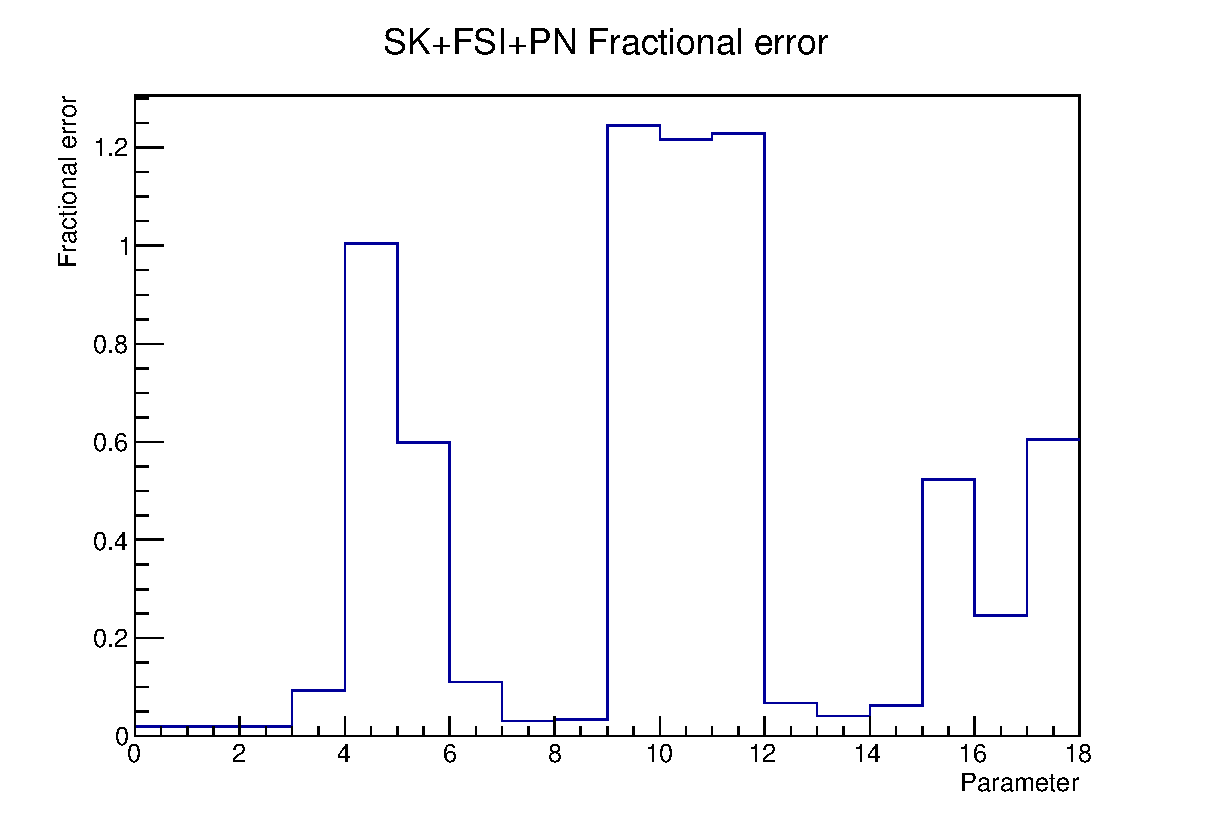
\includegraphics[width=20pc]{./images/systematics/SKFSIPN_frac_error_final.eps}
\caption {
 Values of the fractional errors for each SK+FSI+PN systematic parameter.
}
\label{fig:skfsi_frac}
\end{figure*}
 \begin{figure*}[htb]
\center
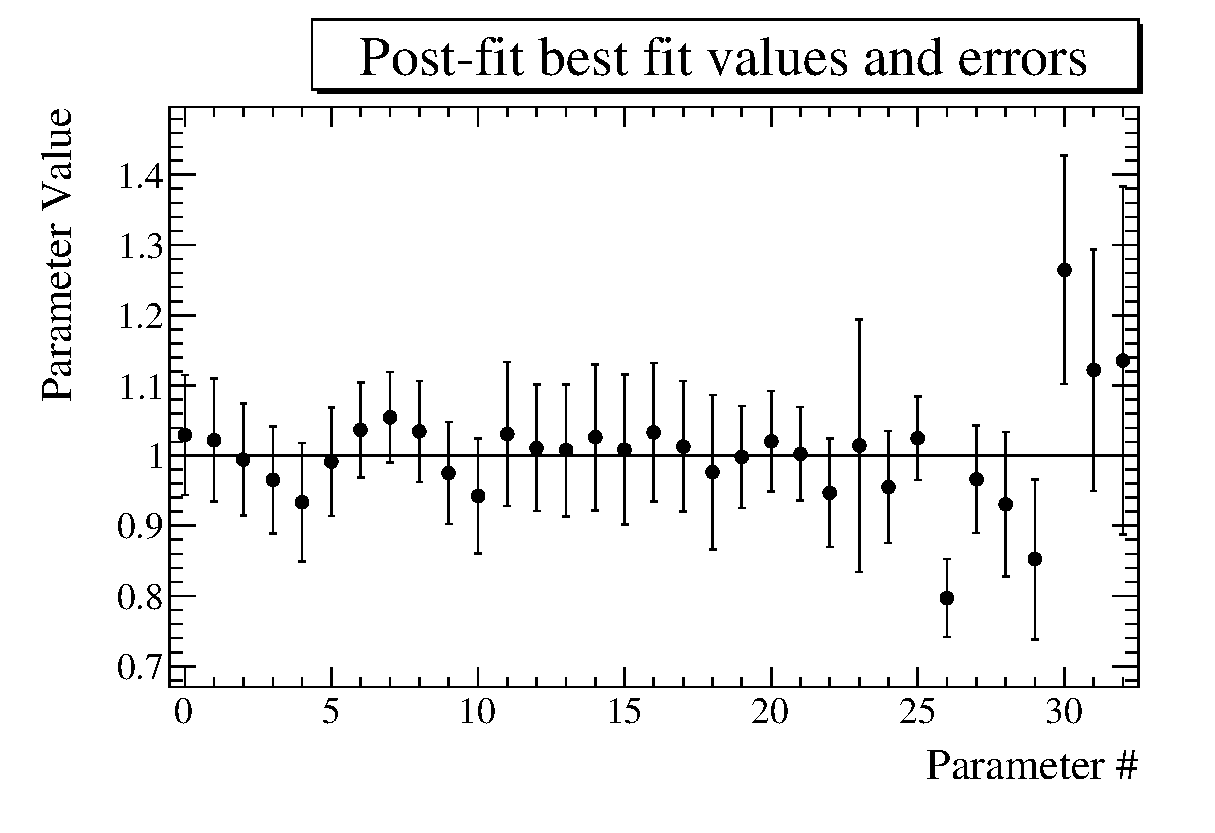
\includegraphics[width=20pc]{./images/systematics/BANFF_postfit_values_errors.eps}
\caption {
 Post-fit values and post-fit fractional errors for each BANFF systematic parameter.
}
\label{fig:banff}
\end{figure*}
\clearpage
{
\tiny
\begin{sideways}
\begin{minipage}{23cm}
{
\setlength{\arraycolsep}{1pt}
\begin{equation}
C^{banff} =\end{equation}
\begin{equation*}
\begin{blockarray}{c p{7pt}p{7pt}p{7pt}p{7pt}p{7pt}p{7pt}p{7pt}p{7pt}p{7pt}p{7pt}p{7pt}p{7pt}p{7pt}p{7pt}p{7pt}p{7pt}p{7pt}p{7pt}p{7pt}p{7pt}p{7pt}p{7pt}p{7pt}p{7pt}p{7pt}p{7pt}p{7pt}p{7pt}p{7pt}p{7pt}p{7pt}p{7pt}p{7pt}}
        & \begin{sideways} {\color{blue} $f_{0; t, r}^{banff}$} \end{sideways} & \begin{sideways} {\color{blue} $f_{1; t, r}^{banff}$} \end{sideways} & \begin{sideways} {\color{blue} $f_{2; t, r}^{banff}$} \end{sideways} & \begin{sideways} {\color{blue} $f_{3; t, r}^{banff}$} \end{sideways} & \begin{sideways} {\color{blue} $f_{4; t, r}^{banff}$} \end{sideways} & \begin{sideways} {\color{blue} $f_{5; t, r}^{banff}$} \end{sideways} & \begin{sideways} {\color{blue} $f_{6; t, r}^{banff}$} \end{sideways} & \begin{sideways} {\color{blue} $f_{7; t, r}^{banff}$} \end{sideways} & \begin{sideways} {\color{blue} $f_{8; t, r}^{banff}$} \end{sideways} & \begin{sideways} {\color{blue} $f_{9; t, r}^{banff}$} \end{sideways} & \begin{sideways} {\color{blue} $f_{10; t, r}^{banff}$} \end{sideways} & \begin{sideways} {\color{blue} $f_{11; t, r}^{banff}$} \end{sideways} & \begin{sideways} {\color{blue} $f_{12; t, r}^{banff}$} \end{sideways} & \begin{sideways} {\color{blue} $f_{13; t, r}^{banff}$} \end{sideways} & \begin{sideways} {\color{blue} $f_{14; t, r}^{banff}$} \end{sideways} & \begin{sideways} {\color{blue} $f_{15; t, r}^{banff}$} \end{sideways} & \begin{sideways} {\color{blue} $f_{16; t, r}^{banff}$} \end{sideways} & \begin{sideways} {\color{blue} $f_{17; t, r}^{banff}$} \end{sideways} & \begin{sideways} {\color{blue} $f_{18; t, r}^{banff}$} \end{sideways} & \begin{sideways} {\color{blue} $f_{19; t, r}^{banff}$} \end{sideways} & \begin{sideways} {\color{blue} $f_{20; t, r}^{banff}$} \end{sideways} & \begin{sideways} {\color{blue} $f_{21; t, r}^{banff}$} \end{sideways} & \begin{sideways} {\color{blue} $f_{22; t, r}^{banff}$} \end{sideways} & \begin{sideways} {\color{blue} $f_{23; t, r}^{banff}$} \end{sideways} & \begin{sideways} {\color{blue} $f_{24; t, r}^{banff}$} \end{sideways} & \begin{sideways} {\color{blue} $f_{25; t, r}^{banff}$} \end{sideways} & \begin{sideways} {\color{blue} $f_{26; t, r}^{banff}$} \end{sideways} & \begin{sideways} {\color{blue} $f_{27; t, r}^{banff}$} \end{sideways} & \begin{sideways} {\color{blue} $f_{28; t, r}^{banff}$} \end{sideways} & \begin{sideways} {\color{blue} $f_{29; t, r}^{banff}$} \end{sideways} & \begin{sideways} {\color{blue} $f_{30; t, r}^{banff}$} \end{sideways} & \begin{sideways} {\color{blue} $f_{31; t, r}^{banff}$} \end{sideways} & \begin{sideways} {\color{blue} $f_{32; t, r}^{banff}$} \end{sideways} \\ 
\begin{block}{c(p{7pt}p{7pt}p{7pt}p{7pt}p{7pt}p{7pt}p{7pt}p{7pt}p{7pt}p{7pt}p{7pt}p{7pt}p{7pt}p{7pt}p{7pt}p{7pt}p{7pt}p{7pt}p{7pt}p{7pt}p{7pt}p{7pt}p{7pt}p{7pt}p{7pt}p{7pt}p{7pt}p{7pt}p{7pt}p{7pt}p{7pt}p{7pt}p{7pt}@{\hspace*{1pt}})}
{\color{blue} f_{0; t, r}^{banff}}  \vspace{0.04cm} & {\color{red} 0.007} &      0.007 &      0.006 &      0.005 &      0.004 &      0.004 &      0.004 &      0.003 &      0.002 &      0.002 &      0.001 &      0.008 &      0.006 &      0.005 &      0.005 &      0.003 &      0.007 &      0.006 &      0.006 &      0.005 &      0.003 &      0.002 &      0.001 &      0.006 &      0.002 &     -0.001 &     -0.000 &     -0.004 &     -0.002 &     -0.001 &     -0.005 &     -0.002 &     -0.004 \\ 
{\color{blue} f_{1; t, r}^{banff}}  \vspace{0.04cm} &      0.007 & {\color{red} 0.008} &      0.007 &      0.005 &      0.005 &      0.005 &      0.004 &      0.003 &      0.002 &      0.002 &      0.001 &      0.006 &      0.005 &      0.004 &      0.004 &      0.002 &      0.006 &      0.007 &      0.006 &      0.005 &      0.003 &      0.002 &      0.001 &      0.005 &      0.002 &     -0.001 &     -0.000 &     -0.005 &     -0.002 &     -0.001 &     -0.006 &     -0.001 &     -0.004 \\ 
{\color{blue} f_{2; t, r}^{banff}}  \vspace{0.04cm} &      0.006 &      0.007 & {\color{red} 0.006} &      0.006 &      0.005 &      0.004 &      0.004 &      0.003 &      0.002 &      0.002 &      0.001 &      0.005 &      0.005 &      0.004 &      0.004 &      0.002 &      0.005 &      0.006 &      0.006 &      0.004 &      0.003 &      0.002 &      0.001 &      0.004 &      0.002 &     -0.001 &     -0.000 &     -0.005 &     -0.003 &     -0.001 &     -0.005 &     -0.001 &     -0.004 \\ 
{\color{blue} f_{3; t, r}^{banff}}  \vspace{0.04cm} &      0.005 &      0.005 &      0.006 & {\color{red} 0.006} &      0.005 &      0.005 &      0.004 &      0.003 &      0.002 &      0.002 &      0.001 &      0.005 &      0.005 &      0.005 &      0.004 &      0.002 &      0.005 &      0.005 &      0.005 &      0.004 &      0.003 &      0.002 &      0.001 &      0.004 &      0.002 &     -0.001 &     -0.000 &     -0.005 &     -0.003 &     -0.001 &     -0.006 &     -0.001 &     -0.004 \\ 
{\color{blue} f_{4; t, r}^{banff}}  \vspace{0.04cm} &      0.004 &      0.005 &      0.005 &      0.005 & {\color{red} 0.007} &      0.006 &      0.004 &      0.003 &      0.002 &      0.002 &      0.001 &      0.004 &      0.004 &      0.004 &      0.003 &      0.001 &      0.005 &      0.004 &      0.005 &      0.004 &      0.002 &      0.002 &      0.001 &      0.004 &      0.001 &     -0.001 &     -0.000 &     -0.005 &     -0.002 &     -0.001 &     -0.007 &     -0.001 &     -0.005 \\ 
{\color{blue} f_{5; t, r}^{banff}}  \vspace{0.04cm} &      0.004 &      0.005 &      0.004 &      0.005 &      0.006 & {\color{red} 0.006} &      0.005 &      0.003 &      0.002 &      0.002 &      0.001 &      0.005 &      0.005 &      0.005 &      0.004 &      0.002 &      0.005 &      0.005 &      0.004 &      0.004 &      0.003 &      0.002 &      0.001 &      0.004 &      0.001 &     -0.000 &     -0.000 &     -0.004 &     -0.003 &     -0.001 &     -0.007 &     -0.001 &     -0.005 \\ 
{\color{blue} f_{6; t, r}^{banff}}  \vspace{0.04cm} &      0.004 &      0.004 &      0.004 &      0.004 &      0.004 &      0.005 & {\color{red} 0.005} &      0.003 &      0.002 &      0.002 &      0.002 &      0.005 &      0.005 &      0.004 &      0.005 &      0.003 &      0.004 &      0.004 &      0.004 &      0.003 &      0.003 &      0.002 &      0.002 &      0.004 &      0.002 &     -0.000 &     -0.000 &     -0.003 &     -0.003 &     -0.001 &     -0.006 &     -0.002 &     -0.004 \\ 
{\color{blue} f_{7; t, r}^{banff}}  \vspace{0.04cm} &      0.003 &      0.003 &      0.003 &      0.003 &      0.003 &      0.003 &      0.003 & {\color{red} 0.004} &      0.003 &      0.002 &      0.001 &      0.004 &      0.003 &      0.003 &      0.003 &      0.001 &      0.003 &      0.003 &      0.003 &      0.003 &      0.003 &      0.003 &      0.001 &      0.003 &      0.002 &     -0.000 &     -0.000 &     -0.002 &     -0.002 &     -0.001 &     -0.003 &     -0.003 &     -0.002 \\ 
{\color{blue} f_{8; t, r}^{banff}}  \vspace{0.04cm} &      0.002 &      0.002 &      0.002 &      0.002 &      0.002 &      0.002 &      0.002 &      0.003 & {\color{red} 0.005} &      0.004 &      0.003 &      0.002 &      0.002 &      0.002 &      0.002 &      0.002 &      0.001 &      0.003 &      0.003 &      0.003 &      0.004 &      0.004 &      0.003 &      0.002 &      0.003 &     -0.000 &     -0.000 &     -0.002 &     -0.001 &     -0.002 &     -0.002 &     -0.005 &     -0.001 \\ 
{\color{blue} f_{9; t, r}^{banff}}  \vspace{0.04cm} &      0.002 &      0.002 &      0.002 &      0.002 &      0.002 &      0.002 &      0.002 &      0.002 &      0.004 & {\color{red} 0.005} &      0.005 &      0.002 &      0.002 &      0.002 &      0.003 &      0.004 &      0.001 &      0.001 &      0.001 &      0.002 &      0.003 &      0.004 &      0.005 &      0.000 &      0.004 &     -0.000 &      0.000 &     -0.001 &     -0.000 &     -0.002 &     -0.001 &     -0.006 &     -0.001 \\ 
{\color{blue} f_{10; t, r}^{banff}}  \vspace{0.04cm} &      0.001 &      0.001 &      0.001 &      0.001 &      0.001 &      0.001 &      0.002 &      0.001 &      0.003 &      0.005 & {\color{red} 0.007} &      0.001 &      0.002 &      0.001 &      0.003 &      0.005 &      0.001 &      0.001 &      0.002 &      0.002 &      0.003 &      0.004 &      0.006 &      0.002 &      0.005 &      0.000 &      0.000 &     -0.001 &      0.000 &     -0.002 &     -0.001 &     -0.005 &     -0.001 \\ 
{\color{blue} f_{11; t, r}^{banff}}  \vspace{0.04cm} &      0.008 &      0.006 &      0.005 &      0.005 &      0.004 &      0.005 &      0.005 &      0.004 &      0.002 &      0.002 &      0.001 & {\color{red} 0.010} &      0.008 &      0.008 &      0.007 &      0.004 &      0.008 &      0.007 &      0.006 &      0.005 &      0.004 &      0.002 &      0.002 &      0.007 &      0.003 &     -0.001 &     -0.000 &     -0.004 &     -0.003 &     -0.000 &     -0.006 &     -0.001 &     -0.004 \\ 
{\color{blue} f_{12; t, r}^{banff}}  \vspace{0.04cm} &      0.006 &      0.005 &      0.005 &      0.005 &      0.004 &      0.005 &      0.005 &      0.003 &      0.002 &      0.002 &      0.002 &      0.008 & {\color{red} 0.008} &      0.008 &      0.007 &      0.004 &      0.007 &      0.006 &      0.005 &      0.005 &      0.003 &      0.002 &      0.002 &      0.007 &      0.003 &     -0.001 &     -0.000 &     -0.004 &     -0.003 &     -0.001 &     -0.006 &     -0.001 &     -0.004 \\ 
{\color{blue} f_{13; t, r}^{banff}}  \vspace{0.04cm} &      0.005 &      0.004 &      0.004 &      0.005 &      0.004 &      0.005 &      0.004 &      0.003 &      0.002 &      0.002 &      0.001 &      0.008 &      0.008 & {\color{red} 0.009} &      0.007 &      0.004 &      0.007 &      0.006 &      0.005 &      0.005 &      0.003 &      0.002 &      0.002 &      0.008 &      0.003 &     -0.001 &     -0.000 &     -0.004 &     -0.003 &     -0.001 &     -0.006 &     -0.001 &     -0.004 \\ 
{\color{blue} f_{14; t, r}^{banff}}  \vspace{0.04cm} &      0.005 &      0.004 &      0.004 &      0.004 &      0.003 &      0.004 &      0.005 &      0.003 &      0.002 &      0.003 &      0.003 &      0.007 &      0.007 &      0.007 & {\color{red} 0.011} &      0.009 &      0.004 &      0.005 &      0.006 &      0.004 &      0.004 &      0.003 &      0.003 &      0.007 &      0.003 &     -0.000 &     -0.000 &     -0.003 &     -0.003 &     -0.000 &     -0.005 &     -0.002 &     -0.004 \\ 
{\color{blue} f_{15; t, r}^{banff}}  \vspace{0.04cm} &      0.003 &      0.002 &      0.002 &      0.002 &      0.001 &      0.002 &      0.003 &      0.001 &      0.002 &      0.004 &      0.005 &      0.004 &      0.004 &      0.004 &      0.009 & {\color{red} 0.011} &      0.002 &      0.002 &      0.004 &      0.002 &      0.003 &      0.003 &      0.004 &      0.004 &      0.004 &     -0.000 &     -0.000 &     -0.001 &     -0.002 &     -0.001 &     -0.002 &     -0.003 &     -0.002 \\ 
{\color{blue} f_{16; t, r}^{banff}}  \vspace{0.04cm} &      0.007 &      0.006 &      0.005 &      0.005 &      0.005 &      0.005 &      0.004 &      0.003 &      0.001 &      0.001 &      0.001 &      0.008 &      0.007 &      0.007 &      0.004 &      0.002 & {\color{red} 0.010} &      0.006 &      0.005 &      0.006 &      0.003 &      0.002 &      0.001 &      0.009 &      0.002 &     -0.001 &     -0.000 &     -0.004 &     -0.003 &     -0.000 &     -0.006 &     -0.002 &     -0.004 \\ 
{\color{blue} f_{17; t, r}^{banff}}  \vspace{0.04cm} &      0.006 &      0.007 &      0.006 &      0.005 &      0.004 &      0.005 &      0.004 &      0.003 &      0.003 &      0.001 &      0.001 &      0.007 &      0.006 &      0.006 &      0.005 &      0.002 &      0.006 & {\color{red} 0.009} &      0.006 &      0.005 &      0.004 &      0.002 &      0.001 &      0.009 &      0.003 &     -0.001 &     -0.000 &     -0.004 &     -0.002 &     -0.001 &     -0.006 &     -0.001 &     -0.004 \\ 
{\color{blue} f_{18; t, r}^{banff}}  \vspace{0.04cm} &      0.006 &      0.006 &      0.006 &      0.005 &      0.005 &      0.004 &      0.004 &      0.003 &      0.003 &      0.001 &      0.002 &      0.006 &      0.005 &      0.005 &      0.006 &      0.004 &      0.005 &      0.006 & {\color{red} 0.012} &      0.006 &      0.005 &      0.003 &      0.002 &      0.008 &      0.002 &     -0.001 &     -0.000 &     -0.005 &     -0.003 &     -0.001 &     -0.006 &     -0.001 &     -0.004 \\ 
{\color{blue} f_{19; t, r}^{banff}}  \vspace{0.04cm} &      0.005 &      0.005 &      0.004 &      0.004 &      0.004 &      0.004 &      0.003 &      0.003 &      0.003 &      0.002 &      0.002 &      0.005 &      0.005 &      0.005 &      0.004 &      0.002 &      0.006 &      0.005 &      0.006 & {\color{red} 0.005} &      0.004 &      0.003 &      0.002 &      0.009 &      0.003 &     -0.001 &     -0.000 &     -0.004 &     -0.002 &     -0.001 &     -0.005 &     -0.002 &     -0.004 \\ 
{\color{blue} f_{20; t, r}^{banff}}  \vspace{0.04cm} &      0.003 &      0.003 &      0.003 &      0.003 &      0.002 &      0.003 &      0.003 &      0.003 &      0.004 &      0.003 &      0.003 &      0.004 &      0.003 &      0.003 &      0.004 &      0.003 &      0.003 &      0.004 &      0.005 &      0.004 & {\color{red} 0.005} &      0.004 &      0.003 &      0.007 &      0.004 &     -0.000 &     -0.000 &     -0.002 &     -0.001 &     -0.002 &     -0.003 &     -0.004 &     -0.002 \\ 
{\color{blue} f_{21; t, r}^{banff}}  \vspace{0.04cm} &      0.002 &      0.002 &      0.002 &      0.002 &      0.002 &      0.002 &      0.002 &      0.003 &      0.004 &      0.004 &      0.004 &      0.002 &      0.002 &      0.002 &      0.003 &      0.003 &      0.002 &      0.002 &      0.003 &      0.003 &      0.004 & {\color{red} 0.004} &      0.004 &      0.003 &      0.004 &     -0.000 &     -0.000 &     -0.002 &     -0.001 &     -0.002 &     -0.002 &     -0.005 &     -0.001 \\ 
{\color{blue} f_{22; t, r}^{banff}}  \vspace{0.04cm} &      0.001 &      0.001 &      0.001 &      0.001 &      0.001 &      0.001 &      0.002 &      0.001 &      0.003 &      0.005 &      0.006 &      0.002 &      0.002 &      0.002 &      0.003 &      0.004 &      0.001 &      0.001 &      0.002 &      0.002 &      0.003 &      0.004 & {\color{red} 0.006} &      0.002 &      0.005 &     -0.000 &      0.000 &     -0.001 &     -0.000 &     -0.002 &     -0.001 &     -0.005 &     -0.001 \\ 
{\color{blue} f_{23; t, r}^{banff}}  \vspace{0.04cm} &      0.006 &      0.005 &      0.004 &      0.004 &      0.004 &      0.004 &      0.004 &      0.003 &      0.002 &      0.000 &      0.002 &      0.007 &      0.007 &      0.008 &      0.007 &      0.004 &      0.009 &      0.009 &      0.008 &      0.009 &      0.007 &      0.003 &      0.002 & {\color{red} 0.032} &      0.006 &     -0.001 &     -0.000 &     -0.003 &     -0.002 &     -0.000 &     -0.005 &     -0.001 &     -0.004 \\ 
{\color{blue} f_{24; t, r}^{banff}}  \vspace{0.04cm} &      0.002 &      0.002 &      0.002 &      0.002 &      0.001 &      0.001 &      0.002 &      0.002 &      0.003 &      0.004 &      0.005 &      0.003 &      0.003 &      0.003 &      0.003 &      0.004 &      0.002 &      0.003 &      0.002 &      0.003 &      0.004 &      0.004 &      0.005 &      0.006 & {\color{red} 0.006} &     -0.000 &      0.000 &     -0.001 &      0.000 &     -0.002 &     -0.001 &     -0.004 &     -0.000 \\ 
{\color{blue} f_{25; t, r}^{banff}}  \vspace{0.04cm} &     -0.001 &     -0.001 &     -0.001 &     -0.001 &     -0.001 &     -0.000 &     -0.000 &     -0.000 &     -0.000 &     -0.000 &      0.000 &     -0.001 &     -0.001 &     -0.001 &     -0.000 &     -0.000 &     -0.001 &     -0.001 &     -0.001 &     -0.001 &     -0.000 &     -0.000 &     -0.000 &     -0.001 &     -0.000 & {\color{red} 0.004} &     -0.001 &     -0.001 &     -0.002 &     -0.002 &      0.001 &      0.002 &      0.001 \\ 
{\color{blue} f_{26; t, r}^{banff}}  \vspace{0.04cm} &     -0.000 &     -0.000 &     -0.000 &     -0.000 &     -0.000 &     -0.000 &     -0.000 &     -0.000 &     -0.000 &      0.000 &      0.000 &     -0.000 &     -0.000 &     -0.000 &     -0.000 &     -0.000 &     -0.000 &     -0.000 &     -0.000 &     -0.000 &     -0.000 &     -0.000 &      0.000 &     -0.000 &      0.000 &     -0.001 & {\color{red} 0.003} &      0.000 &      0.000 &      0.000 &     -0.004 &     -0.004 &     -0.003 \\ 
{\color{blue} f_{27; t, r}^{banff}}  \vspace{0.04cm} &     -0.004 &     -0.005 &     -0.005 &     -0.005 &     -0.005 &     -0.004 &     -0.003 &     -0.002 &     -0.002 &     -0.001 &     -0.001 &     -0.004 &     -0.004 &     -0.004 &     -0.003 &     -0.001 &     -0.004 &     -0.004 &     -0.005 &     -0.004 &     -0.002 &     -0.002 &     -0.001 &     -0.003 &     -0.001 &     -0.001 &      0.000 & {\color{red} 0.006} &      0.004 &      0.002 &      0.005 &      0.000 &      0.003 \\ 
{\color{blue} f_{28; t, r}^{banff}}  \vspace{0.04cm} &     -0.002 &     -0.002 &     -0.003 &     -0.003 &     -0.002 &     -0.003 &     -0.003 &     -0.002 &     -0.001 &     -0.000 &      0.000 &     -0.003 &     -0.003 &     -0.003 &     -0.003 &     -0.002 &     -0.003 &     -0.002 &     -0.003 &     -0.002 &     -0.001 &     -0.001 &     -0.000 &     -0.002 &      0.000 &     -0.002 &      0.000 &      0.004 & {\color{red} 0.011} &      0.005 &      0.001 &     -0.005 &      0.001 \\ 
{\color{blue} f_{29; t, r}^{banff}}  \vspace{0.04cm} &     -0.001 &     -0.001 &     -0.001 &     -0.001 &     -0.001 &     -0.001 &     -0.001 &     -0.001 &     -0.002 &     -0.002 &     -0.002 &     -0.000 &     -0.001 &     -0.001 &     -0.000 &     -0.001 &     -0.000 &     -0.001 &     -0.001 &     -0.001 &     -0.002 &     -0.002 &     -0.002 &     -0.000 &     -0.002 &     -0.002 &      0.000 &      0.002 &      0.005 & {\color{red} 0.013} &     -0.003 &     -0.006 &     -0.002 \\ 
{\color{blue} f_{30; t, r}^{banff}}  \vspace{0.04cm} &     -0.005 &     -0.006 &     -0.005 &     -0.006 &     -0.007 &     -0.007 &     -0.006 &     -0.003 &     -0.002 &     -0.001 &     -0.001 &     -0.006 &     -0.006 &     -0.006 &     -0.005 &     -0.002 &     -0.006 &     -0.006 &     -0.006 &     -0.005 &     -0.003 &     -0.002 &     -0.001 &     -0.005 &     -0.001 &      0.001 &     -0.004 &      0.005 &      0.001 &     -0.003 & {\color{red} 0.027} &      0.011 &      0.020 \\ 
{\color{blue} f_{31; t, r}^{banff}}  \vspace{0.04cm} &     -0.002 &     -0.001 &     -0.001 &     -0.001 &     -0.001 &     -0.001 &     -0.002 &     -0.003 &     -0.005 &     -0.006 &     -0.005 &     -0.001 &     -0.001 &     -0.001 &     -0.002 &     -0.003 &     -0.002 &     -0.001 &     -0.001 &     -0.002 &     -0.004 &     -0.005 &     -0.005 &     -0.001 &     -0.004 &      0.002 &     -0.004 &      0.000 &     -0.005 &     -0.006 &      0.011 & {\color{red} 0.029} &      0.009 \\ 
{\color{blue} f_{32; t, r}^{banff}}  \vspace{0.04cm} &     -0.004 &     -0.004 &     -0.004 &     -0.004 &     -0.005 &     -0.005 &     -0.004 &     -0.002 &     -0.001 &     -0.001 &     -0.001 &     -0.004 &     -0.004 &     -0.004 &     -0.004 &     -0.002 &     -0.004 &     -0.004 &     -0.004 &     -0.004 &     -0.002 &     -0.001 &     -0.001 &     -0.004 &     -0.000 &      0.001 &     -0.003 &      0.003 &      0.001 &     -0.002 &      0.020 &      0.009 & {\color{red} 0.061} \\ 
\end{block}
\label{eq:Cbanff}
\end{blockarray}
\end{equation*}
}
\end{minipage}
\end{sideways}
\normalsize
}





%
% ...............................................................................
% Table summarizing which systematics are applied to which sample
%

\begin{table}[htbp]
\center
\begin{tabular}{|p{1cm}|p{3cm}|p{5.75cm}|p{0.75cm}|p{0.75cm}|p{0.75cm}|p{0.75cm}|p{0.75cm}|}
\hline 
 & & & \multicolumn{2}{c|}{Stand-alone} & \multicolumn{2}{c|}{Joint OA} & \\
Type & Systematics & Comment & $1R_{\mu}$ & $1R_{e}$ & $1R_{\mu}$ & $1R_{e}$ & $N_{syst}$ \\
\hline 
\hline
  \multirow{6}{*} { \begin{sideways} BANFF \end{sideways} } 
       & $f_{0; t, r}^{banff}$ - $f_{24; t, r}^{banff}$          
          & $\nu_{\mu}$  flux &  11 &  11  &  11 & 11 & 25 \\
 
&    &  $\bar{\nu_{\mu}}$  flux &  5 &  2  &  5 & 5 &  \\
&    &  ${\nu_{e}}$  flux &  -- &  7  &  7 &  7 &\\
&    &  $\bar{\nu_{e}}$  flux &  -- &  2  &  2 & 2 & \\
  \cline{2-8}
       & $f_{25; t, r}^{banff}$ 
          & CCQE axial mass                  &  {\ck} &  {\ck} & \ck & \ck & 8 \\
       & $f_{26; t, r}^{banff}$ 
          & resonance-production axial mass  &  {\ck} &  {\ck} & \ck & \ck & \\
       & $f_{27; t, r}^{banff}$ - $f_{29; t, r}^{banff}$  
          & CCQE normalization            &  3 &  1 & 3 & 3 & \\
       & $f_{30; t, r}^{banff}$ - $f_{31; t, r}^{banff}$ 
          & CC1$\pi$ normalization        &  2 &  1 & 2 &  2 & \\
       & $f_{32; t, r}^{banff}$ 
          & NC1$\pi^{0}$                  &   --               &  \ck               & -- & \ck & \\
\hline
  \multirow{12}{*} {  \begin{sideways} Uncorrelated cross-section \end{sideways} } 
       & $f_{pF; t, r}$ 
          & Fermi momentum           &  {\ck} &  {\ck} & \ck & \ck &12 \\
       & $f_{bindE; t, r}$ 
         & Binding energy            &  {\ck} &  -- & \ck & \ck & \\
       & $f_{SF; t, r}$
         & Nuclear modeling          &  {\ck} &  {\ck} & \ck &  \ck &  \\
       & $f_{Wshape; t, r}$
         & Shape of the $\pi$ momentum distribution    &  {\ck} &  {\ck} & \ck & \ck & \\
       & $f_{\pi-less\Delta; t, r}$
         & $\pi$-less $\Delta$ decay    &  {\ck} &  {\ck} & \ck &  \ck & \\
       & $f_{CCothShape; t, r}$
         & CC other shape               &  {\ck} &  {\ck} & \ck & \ck & \\
       & $f_{CCcoh; t}$
         & CC coherent cross-section    & {\ck} &  {\ck} & \ck & \ck &  \\
       & $f_{NC1\pi^\pm; t}$
         & NC1$\pi^{\pm}$ cross-section & \ck & -- & \ck & -- &\\
       & $f_{NCcoh; t}$
         & NC coherent cross-section    & -- & \ck & -- & \ck & \\
       & $f_{NCoth; t}$
         & NC other cross-section       & {\ck} &  {\ck} & \ck & \ck & \\
       & $f_{CC\nu_e; t}$
         & $\sigma_{\nu_{e}}$/ $\sigma_{\nu_{\mu}}$ ratio & {\ck} &  {\ck} & \ck & \ck & \\
       & $f_{CC\bar{\nu}; t}$
         & $\sigma_{\bar{\nu}}$/ $\sigma_{\nu}$ ratio      & {\ck} &  -- & \ck & \ck & \\
\hline 
\hline
   \multirow{3}{*} { \begin{sideways} SK + FSI\end{sideways} } 
      & $f_{E; r}^{SK}$  
          & Reconstructed energy scale & {\ck}  &  {\ck}  & \ck & \ck & 1 \\
   \cline{2-8}
      & $f_{0; r}^{SK+FSI}$-$f_{5; r}^{SK+FSI}$ 
          &  $1R_{\mu}$ efficiencies  & \ck & -- &  \ck & --& 6  \\
   \cline{2-8}
       & $f_{6; r}^{SK+FSI}$-$f_{17; r}^{SK+FSI}$ 
          &  $1R_{e}$ efficiencies  & -- & \ck &  -- & \ck & 12 \\
 \hline 
\hline
\bf Total &  &  & \bf 41 & \bf 49 & \multicolumn{2}{|c|}{\bf 64} & \\
\hline
\end{tabular}
\caption{
  List of all systematic parameters included in the joint oscillation analysis.
  A \ck symbol indicates whether the systematic parameter is applied on the single $\mu$-like ring 
  and single e-like ring MC templates.
}
\label{tab:apply_syst_to_samples}
\end{table}




% .................
\clearpage
% ........................................
%
% table showing which systematics are applied to which 1Rmu modes
%

{
\setlength{\tabcolsep}{2pt}
\renewcommand{\arraystretch}{1.5}
\begin{table}
\scriptsize
\centering
\begin{tabular}{| c || c | c | c | c | c | c || c | c | c | c | c | c || c | c | c | c | c | c || c | c | c | c | c | c || c | c | c | c || c | c | c | c || c | c | c | c |}
\hline
                       & \begin{sideways}   $\nu_{\mu}$ CCQE                   \end{sideways}  &   
                         \begin{sideways}   $\nu_{\mu}$ CC1$\pi$               \end{sideways}  &   
                         \begin{sideways}   $\nu_{\mu}$ CC coherent            \end{sideways}  &   
                         \begin{sideways}   $\nu_{\mu}$ CC other               \end{sideways}  &   
                         \begin{sideways}   $\nu_{\mu}$ NC1$\pi^{\pm}$         \end{sideways}  &  
                         \begin{sideways}   $\nu_{\mu}$ NC other               \end{sideways}  &   
                         \begin{sideways}   $\bar{\nu_{\mu}}$ CCQE             \end{sideways}  &  
                         \begin{sideways}   $\bar{\nu_{\mu}}$ CC1$\pi$         \end{sideways}  &  
                         \begin{sideways}   $\bar{\nu_{\mu}}$ CC coherent      \end{sideways}  &  
                         \begin{sideways}   $\bar{\nu_{\mu}}$ CC other         \end{sideways}  &  
                         \begin{sideways}   $\bar{\nu_{\mu}}$ NC1$\pi^{\pm}$   \end{sideways}  &   
                         \begin{sideways}   $\bar{\nu_{\mu}}$ NC other         \end{sideways}  &   
                         \begin{sideways}   $\nu_{e}$ CCQE                     \end{sideways}  &   
                         \begin{sideways}   $\nu_{e}$ CC1$\pi$                 \end{sideways}  &   
                         \begin{sideways}   $\nu_{e}$ CC coherent              \end{sideways}  &  
                         \begin{sideways}   $\nu_{e}$ CC other                 \end{sideways}  &   
                         \begin{sideways}   $\nu_{e}$ NC1$\pi^{\pm}$           \end{sideways}  &   
                         \begin{sideways}   $\nu_{e}$ NC other                 \end{sideways}  &  
                         \begin{sideways}   $\bar{\nu_{e}}$ CCQE               \end{sideways}  &   
                         \begin{sideways}   $\bar{\nu_{e}}$ CC1$\pi$           \end{sideways}  &   
                         \begin{sideways}   $\bar{\nu_{e}}$ CC coherent        \end{sideways}  &   
                         \begin{sideways}   $\bar{\nu_{e}}$ CC other           \end{sideways}  &  
                         \begin{sideways}   $\bar{\nu_{e}}$ NC1$\pi^{\pm}$     \end{sideways}  & 
                         \begin{sideways}   $\bar{\nu_{e}}$ NC other           \end{sideways}  &   
                         \begin{sideways}   Osc-$\nu_{e}$ CCQE                 \end{sideways}  &   
                         \begin{sideways}   Osc-$\nu_{e}$ CC1$\pi$             \end{sideways}  &   
                         \begin{sideways}   Osc-$\nu_{e}$ CC coherent          \end{sideways}  &   
                         \begin{sideways}   Osc-$\nu_{e}$ CC other             \end{sideways}  &
                           \begin{sideways}   Osc-$\nu_{\mu}$ CCQE                 \end{sideways}  &   
                         \begin{sideways}   Osc-$\nu_{\mu}$ CC1$\pi$             \end{sideways}  &   
                         \begin{sideways}   Osc-$\nu_{\mu}$ CC coherent          \end{sideways}  &   
                         \begin{sideways}   Osc-$\nu_{\mu}$ CC other             \end{sideways}  &
                           \begin{sideways}   Osc-$\bar{\nu_{e}}$ CCQE                 \end{sideways}  &   
                         \begin{sideways}   Osc-$\bar{\nu_{e}}$ CC1$\pi$             \end{sideways}  &   
                         \begin{sideways}   Osc-$\bar{\nu_{e}}$ CC coherent          \end{sideways}  &   
                         \begin{sideways}   Osc-$\bar{\nu_{e}}$ CC other             \end{sideways}  \\
\hline
 $f_{E; r}^{SK}$             & \ck & \ck & \ck & \ck & \ck & \ck & \ck & \ck & \ck & \ck & \ck & \ck & \ck & \ck & \ck & \ck & \ck & \ck & \ck & \ck & \ck & \ck & \ck & \ck & \ck & \ck & \ck & \ck  & \ck & \ck & \ck & \ck & \ck & \ck & \ck & \ck \\
\hline
 $f_{0; t, r}^{banff}$ -
 $f_{10; t, r}^{banff}$      & \ck & \ck & \ck & \ck & \ck & \ck &     &     &     &     &     &     &     &     &     &     &     &     &     &     &     &     &     &   & \ck & \ck & \ck & \ck &   &    &     &     &  & & &    \\ 
\hline
 $f_{11; t, r}^{banff}$ -   
 $f_{15; t, r}^{banff}$      &     &     &     &     &     &     & \ck & \ck & \ck & \ck & \ck & \ck &     &     &     &     &     &     &     &     &     &     &     &     &     &     &     &    & & & & &\ck & \ck & \ck & \ck   \\
\hline
 $f_{16; t, r}^{banff}$ -   
 $f_{22; t, r}^{banff}$      &     &     &     &     &     &     &     &     &     &     &     &     & \ck & \ck & \ck & \ck & \ck & \ck &     &     &     &     &     &     &     &     &     &    & \ck & \ck & \ck & \ck  & & & & \\
\hline
 $f_{23; t, r}^{banff}$ -   
 $f_{24; t, r}^{banff}$      &     &     &     &     &     &     &     &     &     &     &     &     &     &     &     &     &     &   & \ck & \ck & \ck & \ck & \ck & \ck &    &     &     &   & & & & & & & &    \\
\hline
 $f_{25; t, r}^{banff}$      & \ck &     &     &     &     &     & \ck &     &     &     &     &     & \ck &     &     &     &     &     & \ck &     &     &     &     &     & \ck &     &     &  & \ck &     &     &  & \ck &     &     &       \\
\hline
 $f_{26; t, r}^{banff}$      &     & \ck &     & \ck & \ck & \ck &     & \ck &     & \ck & \ck & \ck &     & \ck &     & \ck & \ck & \ck &     & \ck &     & \ck & \ck & \ck &     &\ck  &     & \ck &     &\ck  &     & \ck &     &\ck  &     & \ck  \\
\hline
 $f_{27; t, r}^{banff}$      & \ck &     &     &     &     &     & \ck &     &     &     &     &     & \ck &     &     &     &     &     & \ck &     &     &     &     &     & \ck &     &     &  & \ck &     &     &  & \ck &     &     &       \\
\hline
 $f_{28; t, r}^{banff}$      & \ck &     &     &     &     &     & \ck &     &     &     &     &     & \ck &     &     &     &     &     & \ck &     &     &     &     &     & \ck &     &     &  & \ck &     &     &  & \ck &     &     &       \\
\hline
 $f_{29; t, r}^{banff}$      & \ck &     &     &     &     &     & \ck &     &     &     &     &     & \ck &     &     &     &     &     & \ck &     &     &     &     &     & \ck &     &     &  & \ck &     &     &  & \ck &     &     &       \\
\hline
 $f_{30; t, r}^{banff}$      &     & \ck &     &     &     &     &     & \ck &     &     &     &     &     & \ck &     &     &     &     &     & \ck &     &     &     &     &     & \ck &     &      &     & \ck &     &       &     & \ck &     &      \\
\hline
 $f_{31; t, r}^{banff}$      &     & \ck &     &     &     &     &     & \ck &     &     &     &     &     & \ck &     &     &     &     &     & \ck &     &     &     &     &     & \ck &     &       &     & \ck &     &       &     & \ck &     &   \\
\hline
$f_{32; t, r}^{banff}$      &     &  &     &     &     &     &     &  &     &     &     &     &     &  &     &     &     &     &     &  &     &     &     &     &     &  &     &       &     &  &     &       &     &  &     &   \\
\hline
 $f_{pF; t, r}$               & \ck &     &     &     &     &     & \ck &     &     &     &     &     & \ck &     &     &     &     &     & \ck &     &     &     &     &     & \ck &     &     &  & \ck &     &     &  & \ck &     &     &       \\
\hline
 $f_{SF; t, r}$               & \ck &     &     &     &     &     & \ck &     &     &     &     &     & \ck &     &     &     &     &     & \ck &     &     &     &     &     & \ck &     &     &  & \ck &     &     &  & \ck &     &     &       \\
\hline
 $f_{bindE; t, r}$           & \ck &     &     &     &     &     & \ck &     &     &     &     &     & \ck &     &     &     &     &     & \ck &     &     &     &     &     & \ck &     &     &  & \ck &     &     &  & \ck &     &     &       \\
\hline
 $f_{\pi-less\Delta; t, r}$  &     &\ck  &     &     & \ck & \ck &     & \ck &     &     & \ck & \ck &     & \ck &     &     &\ck  &\ck  &     & \ck &     &     & \ck & \ck &     & \ck &     &     &     & \ck &     &     &     & \ck &     &      \\
\hline
 $f_{CCothShape; t, r}$      &     &     &     &\ck  &     &     &     &     &     & \ck &     &     &     &     &     & \ck &     &     &     &     &     & \ck &     &     &     &     &     & \ck&     &     &     & \ck &     &     &     & \ck  \\
\hline
 $f_{Wshape; t, r}$          &     &     &     &     & \ck & \ck &     &     &     &     &\ck  & \ck &     &     &     &     & \ck & \ck &     &     &     &     &\ck  & \ck &     &     &     &  &     &     &     &  &     &     &     &      \\
\hline
 $f_{CCcoh; t}$              &     &     & \ck &     &     &     &     &     & \ck &     &     &     &     &     & \ck &     &     &     &     &     & \ck &     &     &     &     &     & \ck &      &     &     & \ck &       &     &     & \ck &      \\
\hline
 $f_{NC1\pi^\pm; t}$         &     &     &     &     & \ck &     &     &     &     &     & \ck &     &     &     &     &     & \ck &     &     &     &     &     & \ck &     &     &     &     &    &     &     &     &    &     &     &     &      \\
\hline
 $f_{NCcoh; t}$  &     &  &     &     &     &     &     &  &     &     &     &     &     &  &     &     &     &     &     &  &     &     &     &     &     &  &     &       &     &  &     &       &     &  &     &   \\
\hline
 $f_{NCoth; t}$              &     &     &     &     &     & \ck &     &     &     &     &     & \ck &     &     &     &     &     & \ck &     &     &     &     &     &\ck  &     &     &     & &     &     &     & &     &     &     &      \\
\hline
 $f_{CC\nu_e; t}$            &     &     &     &     &     &     &     &     &     &     &     &     & \ck & \ck & \ck &\ck  &     &     &\ck  &\ck  & \ck & \ck &     &     & \ck & \ck & \ck & \ck &     &     &     &     & \ck & \ck & \ck & \ck\\
\hline
 $f_{CC\bar{\nu}; t}$        &     &     &     &     &     &     & \ck & \ck & \ck & \ck &     &     &     &     &     &     &     &     & \ck & \ck & \ck & \ck &     &     &     &     &     &  &     &     &     &     & \ck & \ck & \ck & \ck   \\
\hline
 $f _{0; r}^{SK+FSI}$      & \ck &     &     &     &     &     & \ck &     &     &     &     &     &     &     &     &     &     &     &     &     &     &     &     &     &     &     &     &    & \ck &     &     &     &     &     &     &    \\
\hline
 $f _{1; r}^{SK+FSI}$      & \ck &     &     &     &     &     & \ck &     &     &     &     &     &     &     &     &     &     &     &     &     &     &     &     &     &     &     &     &    & \ck &     &     &     &     &     &     &  \\
\hline
 $f _{2; r}^{SK+FSI}$      & \ck &     &     &     &     &     & \ck &     &     &     &     &     &     &     &     &     &     &     &     &     &     &     &     &     &     &     &     &    & \ck &     &     &     &     &     &     &      \\
\hline
 $f _{3; r}^{SK+FSI}$      &     & \ck & \ck & \ck &     &     &     & \ck & \ck & \ck &     &     &     &     &     &     &     &     &     &     &     &     &     &     &     &     &     &    &     & \ck & \ck & \ck  &     &     &     &   \\
\hline
 $f _{4; r}^{SK+FSI}$      &     &     &     &     &     &     &     &     &     &     &     &     & \ck & \ck & \ck & \ck &     &     & \ck & \ck & \ck & \ck &     &     & \ck & \ck & \ck & \ck  &     &     &     &  & \ck & \ck & \ck & \ck\\
\hline
 $f _{5; r}^{SK+FSI}$      &     &     &     &     & \ck & \ck &     &     &     &     & \ck & \ck &     &     &     &     & \ck & \ck &     &     &     &     & \ck & \ck &     &     &     & &     &     &     & &     &     &     &      \\
\hline
$f _{6; r}^{SK+FSI}$-$f _{17; r}^{SK+FSI}$ &     &  &     &     &     &     &     &  &     &     &     &     &     &  &     &     &     &     &     &  &     &     &     &     &     &  &     &       &     &  &     &       &     &  &     &   \\
\hline
\end{tabular}
\caption{
  A \ck symbol denotes that the given single $\mu$-like ring MC template is modified when the given systematic parameter is tweaked.
  The table lists all systematic parameters considered in this analysis (first column),
and all 36 MC templates used for constructing the single $\mu$-like ring event reconstructed energy spectrum p.d.f (first row).
}
\label{tab:apply_syst_to_1Rmu_templates}
\end{table}
}




\clearpage
% ........................................
%
% table showing which systematics are applied to which 1Re modes
%

{
\setlength{\tabcolsep}{2pt}
\renewcommand{\arraystretch}{1.4}
\begin{table}
\scriptsize
\centering
\begin{tabular}{| c || c | c | c | c | c | c | c || c | c | c | c | c | c | c || c | c | c | c | c | c | c || c | c | c | c | c | c | c || c | c | c | c || c | c | c | c || c | c | c | c |}
\hline
                       & \begin{sideways}   $\nu_{\mu}$ CCQE                   \end{sideways}  &   
                         \begin{sideways}   $\nu_{\mu}$ CC1$\pi$               \end{sideways}  &   
                         \begin{sideways}   $\nu_{\mu}$ CC coherent            \end{sideways}  &   
                         \begin{sideways}   $\nu_{\mu}$ CC other               \end{sideways}  &   
                         \begin{sideways}   $\nu_{\mu}$ NC1$\pi^{0}$           \end{sideways}  &  
                         \begin{sideways}   $\nu_{\mu}$ NC coherent            \end{sideways}  &  
                         \begin{sideways}   $\nu_{\mu}$ NC other               \end{sideways}  &   
                         \begin{sideways}   $\bar{\nu_{\mu}}$ CCQE             \end{sideways}  &  
                         \begin{sideways}   $\bar{\nu_{\mu}}$ CC1$\pi$         \end{sideways}  &  
                         \begin{sideways}   $\bar{\nu_{\mu}}$ CC coherent      \end{sideways}  &  
                         \begin{sideways}   $\bar{\nu_{\mu}}$ CC other         \end{sideways}  &  
                         \begin{sideways}   $\bar{\nu_{\mu}}$ NC1$\pi^{0}$     \end{sideways}  &   
                         \begin{sideways}   $\bar{\nu_{\mu}}$ NC coherent      \end{sideways}  &   
                         \begin{sideways}   $\bar{\nu_{\mu}}$ NC other         \end{sideways}  & 
                         \begin{sideways}   $\nu_{e}$ CCQE                     \end{sideways}  &   
                         \begin{sideways}   $\nu_{e}$ CC1$\pi$                 \end{sideways}  &   
                         \begin{sideways}   $\nu_{e}$ CC coherent              \end{sideways}  &  
                         \begin{sideways}   $\nu_{e}$ CC other                 \end{sideways}  &   
                         \begin{sideways}   $\nu_{e}$ NC1$\pi^{0}$             \end{sideways}  &   
                         \begin{sideways}   $\nu_{e}$ NC coherent              \end{sideways}  &   
                         \begin{sideways}   $\nu_{e}$ NC other                 \end{sideways}  &  
                         \begin{sideways}   $\bar{\nu_{e}}$ CCQE               \end{sideways}  &   
                         \begin{sideways}   $\bar{\nu_{e}}$ CC1$\pi$           \end{sideways}  &   
                         \begin{sideways}   $\bar{\nu_{e}}$ CC coherent        \end{sideways}  &   
                         \begin{sideways}   $\bar{\nu_{e}}$ CC other           \end{sideways}  &  
                         \begin{sideways}   $\bar{\nu_{e}}$ NC1$\pi^{0}$       \end{sideways}  & 
                         \begin{sideways}   $\bar{\nu_{e}}$ NC coherent        \end{sideways}  &   
                         \begin{sideways}   $\bar{\nu_{e}}$ NC other           \end{sideways}  &   
                         \begin{sideways}   Osc-$\nu_{e}$ CCQE                 \end{sideways}  &   
                         \begin{sideways}   Osc-$\nu_{e}$ CC1$\pi$             \end{sideways}  &   
                         \begin{sideways}   Osc-$\nu_{e}$ CC coherent          \end{sideways}  &   
                         \begin{sideways}   Osc-$\nu_{e}$ CC other             \end{sideways}  &
 			  \begin{sideways}   Osc-$\nu_{\mu}$ CCQE                 \end{sideways}  &   
                         \begin{sideways}   Osc-$\nu_{\mu}$ CC1$\pi$             \end{sideways}  &   
                         \begin{sideways}   Osc-$\nu_{\mu}$ CC coherent          \end{sideways}  &   
                         \begin{sideways}   Osc-$\nu_{\mu}$ CC other             \end{sideways}  &
                         \begin{sideways}   Osc-$\bar{\nu_{e}}$ CCQE                 \end{sideways}  &   
                         \begin{sideways}   Osc-$\bar{\nu_{e}}$ CC1$\pi$             \end{sideways}  &   
                         \begin{sideways}   Osc-$\bar{\nu_{e}}$ CC coherent          \end{sideways}  &   
                         \begin{sideways}   Osc-$\bar{\nu_{e}}$ CC other             \end{sideways}  \\
\hline
 $f_{E; r}^{SK}$             & \ck & \ck & \ck & \ck & \ck & \ck & \ck & \ck & \ck & \ck & \ck & \ck & \ck & \ck & \ck & \ck & \ck & \ck & \ck & \ck & \ck & \ck & \ck & \ck & \ck & \ck & \ck & \ck & \ck & \ck & \ck & \ck & \ck & \ck & \ck & \ck& \ck & \ck & \ck & \ck \\
\hline
  $f_{0; t, r}^{banff}$ -
 $f_{10; t, r}^{banff}$      & \ck & \ck & \ck & \ck & \ck & \ck & \ck &     &     &     &     &     &     &     &     &     &     &     &     &     &     &     &     &     &     &     &     &    & \ck & \ck & \ck & \ck &   &    &     &     &  & & &    \\ 
\hline
 $f_{11; t, r}^{banff}$ -   
 $f_{15; t, r}^{banff}$      &     &     &     &     &     &     &     & \ck & \ck & \ck & \ck & \ck & \ck & \ck &     &     &     &     &     &     &     &     &     &     &     &     &     &     &     &     &     &   &     &     &     &     & \ck & \ck & \ck & \ck \\
\hline
 $f_{16; t, r}^{banff}$ -   
 $f_{22; t, r}^{banff}$      &     &     &     &     &     &     &     &     &     &     &     &     &     &     & \ck & \ck & \ck & \ck & \ck & \ck & \ck &     &     &     &     &     &     &     &     &     &     &    & \ck & \ck & \ck & \ck  &     &     &     &  \\
\hline
 $f_{23; t, r}^{banff}$ -   
 $f_{24; t, r}^{banff}$      &     &     &     &     &     &     &     &     &     &     &     &     &     &     &     &     &     &     &     &     &     & \ck & \ck & \ck & \ck &  \ck    & \ck & \ck &     &     &     &    &     &   &     & &     &   &     &   \\
\hline
 $f_{25; t, r}^{banff}$      & \ck &     &     &     &     &     &     & \ck &     &     &     &     &     &     & \ck &     &     &     &     &     &     & \ck &     &     &     &     &     &     & \ck &     &     &  & \ck &     &     & & \ck &     &     &    \\
\hline
 $f_{26; t, r}^{banff}$      &     & \ck &     & \ck & \ck &  & \ck &     & \ck &     & \ck & \ck &  & \ck &     & \ck &     & \ck & \ck &  & \ck &     & \ck &     & \ck &   \ck &  & \ck &     &\ck  &     & \ck &     &\ck  &     & \ck &     &\ck  &     & \ck  \\
\hline
 $f_{27; t, r}^{banff}$      & \ck &     &     &     &     &     &     & \ck &     &     &     &     &     &     & \ck &     &     &     &     &     &     & \ck &     &     &     &     &     &     & \ck &     &     &    & \ck &     &     &     & \ck &     &     &      \\
\hline
 $f_{28; t, r}^{banff}$      & \ck &     &     &     &     &     &     & \ck &     &     &     &     &     &     & \ck &     &     &     &     &     &     & \ck &     &     &     &     &     &     & \ck &     &     &     & \ck &     &     &     & \ck &     &     &     \\
\hline
 $f_{29; t, r}^{banff}$      & \ck &     &     &     &     &     &     & \ck &     &     &     &     &     &     & \ck &     &     &     &     &     &     & \ck &     &     &     &     &     &     & \ck &     &     &    & \ck &     &     &     & \ck &     &     &      \\
\hline
 $f_{30; t, r}^{banff}$      &     & \ck &     &     &     &     &     &     & \ck &     &     &     &     &     &     & \ck &     &     &     &     &     &     & \ck &     &     &     &     &     &     & \ck &     &  &     & \ck &     &  &     & \ck &     &      \\
\hline
 $f_{31; t, r}^{banff}$     &     & \ck &     &     &     &     &     &     & \ck &     &     &     &     &     &     & \ck &     &     &     &     &     &     & \ck &     &     &     &     &     &     & \ck &     &  &     & \ck &     &  &     & \ck &     &      \\
\hline
 $f_{32; t, r}^{banff}$      &     &   &     &     &   \ck  &     &     &     &   &     &     &   \ck  &     &   &     &   &     &     &   \ck  &     &   &     &   &     &     &   \ck  &     &   &     &     &     &   &     &     &     &   &     &     &     &  \\
\hline
 $f_{pF; t, r}$              & \ck &     &     &     &     &     &     & \ck &     &     &     &     &     &     & \ck &     &     &     &     &     &     & \ck &     &     &     &     &     &     & \ck &     &     &  & \ck &     &     &   & \ck &     &     &      \\
\hline
 $f_{SF; t, r}$              & \ck &     &     &     &     &     &     & \ck &     &     &     &     &     &     & \ck &     &     &     &     &     &     & \ck &     &     &     &     &     &     & \ck &     &     &   & \ck &     &     &   & \ck &     &     &     \\
\hline
 $f_{bindE; t, r}$         & \ck &     &     &     &     &     &     & \ck &     &     &     &     &     &     & \ck &     &     &     &     &     &     & \ck &     &     &     &     &     &     & \ck &     &     &    & \ck &     &     &   & \ck &     &     &   \\
\hline
 $f_{\pi-less\Delta; t, r}$  &     &\ck  &     &     & \ck &     & \ck &     & \ck &     &     & \ck &     & \ck &     & \ck &     &    &\ck  &  & \ck &     & \ck &     &     & \ck &    & \ck &     & \ck &     &    &     & \ck &     &     &     & \ck &     &      \\
\hline
 $f_{CCothShape; t, r}$      &     &     &     &\ck  &     &     &     &     &     &     & \ck &     &     &     &     &     &     & \ck &     &     &     &     &     &     & \ck &     &     &     &     &     &     & \ck  &     &     &     & \ck   &     &     &     & \ck  \\
\hline
 $f_{Wshape; t, r}$          &     &     &     &     & \ck &     & \ck &     &     &     &     &\ck  &     & \ck &     &     &     &     &   \ck  &  & \ck &     &     &     &     &    \ck &  & \ck &     &     &     &    &     &     &     &     &     &     &     &      \\
\hline
 $f_{CCcoh; t}$              &     &     & \ck &     &     &     &     &     &     & \ck &     &     &     &     &     &     & \ck &     &     &     &     &     &     & \ck &     &     &     &     &     &     & \ck & &     &     & \ck & &     &     & \ck &      \\
\hline
$f_{NC1\pi^\pm; t}$          &     &     &     &     &  &     &     &     &     &     &     &  &     &     &     &     &     &     &     &  &     &     &     &     &     &     &  &     &     &     &     &   &     &     &     &   &     &     &     &      \\
\hline
 $f_{NCcoh; t}$              &     &     &     &     &    & \ck &   &  &     &     &     &    & \ck &     &     &     &     &     &     & \ck &     &     &     &     &     &     &\ck  &     &     &     &  &   &     &     &  &   &     &     &  &    \\
\hline
 $f_{NCoth; t}$              &     &     &     &     &     &     & \ck &     &     &     &     &     &     & \ck &     &     &     &     &     &     & \ck &     &     &     &     &     &     &\ck  &     &     &     &     &     &     &     &     &     &     &     &      \\
\hline
 $f_{CC\nu_e; t}$            &     &     &     &     &     &     &     &     &     &     &     &     &     &     & \ck & \ck & \ck &\ck  &     &     &     &\ck  &\ck  & \ck & \ck &     &     &     & \ck & \ck & \ck & \ck  &     &     &     &  & \ck & \ck & \ck & \ck \\
\hline
 $f_{CC\bar{\nu}; t}$        &     &     &     &     &     &     &     & \ck & \ck & \ck & \ck &     &     &     &     &     &     &     &     &     &     & \ck & \ck & \ck & \ck &     &     &     &     &     &     &     &     &     &     &    & \ck & \ck & \ck & \ck \\
\hline
$f _{0; r}^{SK+FSI}$- $f _{5; r}^{SK+FSI}$  &     &     &     &     &  &     &     &     &     &     &     &  &     &     &     &     &     &     &     &  &     &     &     &     &     &     &  &     &     &     &     &   &     &     &     &   &     &     &     &      \\
\hline
$f _{6; r}^{SK+FSI}$- $f _{8; r}^{SK+FSI}$  &     &     &     &     &     &     &     &     &     &     &     &     &     &     &     &     &     &     &     &     &     &     &     &     &     &     &     &     & \ck & \ck & \ck & \ck  &     &     &     &    &     &     &     &   \\
\hline
$f _{9; r}^{SK+FSI}$- $f _{11; r}^{SK+FSI}$  & \ck & \ck & \ck & \ck &     &     &     & \ck & \ck & \ck & \ck &     &     &     &     &     &     &     &     &     &     &     &     &     &     &     &     &     &     &     &     &    & \ck & \ck & \ck & \ck  &     &     &     &     \\
\hline
$f _{12; r}^{SK+FSI}$- $f _{14; r}^{SK+FSI}$   &     &     &     &     &     &     &     &     &     &     &     &     &     &     & \ck & \ck & \ck & \ck &     &     &     & \ck & \ck & \ck & \ck &     &     &     &     &     &     &    &     &     &     &    & \ck & \ck & \ck & \ck    \\
\hline
$f _{15; r}^{SK+FSI}$- $f _{17; r}^{SK+FSI}$    &     &     &     &     & \ck & \ck & \ck &     &     &     &     & \ck & \ck & \ck &     &     &     &     & \ck & \ck & \ck &     &     &     &     & \ck & \ck & \ck  &     &     &     &     &     &     &     &   &     &     &     &    \\
\hline
\end{tabular}
\caption{
  A \ck symbol denotes that the given single e-like ring MC template is modified when the given systematic parameter is tweaked.
  The table lists all systematic parameters considered in this analysis (first column) and 
  all 40 MC templates used for constructing the single e-like ring event reconstructed energy spectrum p.d.f (first row).
}
\label{tab:apply_syst_to_1Re_templates}
\end{table}
}


\clearpage





%%%%% EVALUATION

\subsection {Evaluation of effects of systematic parameters on the predicted single $\mu$-like ring and single e-like ring reconstructed energy spectra and number of events}
\label{sec:systematics:evaluation}


In this section,  the effects of the systematics described in Sec. \ref{sec:systematics}
on the predicted number of single $\mu$-like ring events and single e-like ring events, 
and the predicted reconstructed energy spectra in SuperK will be evaluated. 

The effects of systematic uncertainties on the predicted number of events are summarised in Tab.\ \ref{tab:systematics:nsk_table_summary}, 
for oscillations with 
$\sin^{2}\theta_{12}$=0.306,	
 $\sin^{2}\theta_{13}$=0.0251,
 $\sin^{2}\theta_{23}$=0.5,
 $\delta m^{2}$=7.5$\times10^{-5}$ $eV^{2}/c^{4}$,
   $|\Delta m^{2}|$=2.4375$\times10^{-3}$ $eV^{2}/c^{4}$,
  $\delta_{CP}$=0 and 
  with the normal mass hierarchy assumed.
In this table, systematic parameters are grouped into four categories
(BANFF, uncorrelated cross sections, SK+FSI errors and total)
 and all parameter correlations are taken into account.
Percentage uncertainties are given,
computed throwing $10^{6}$ toy experiments, varying only the systematics in the selected category
(fixing the rest to their nominal value) and finding the RMS/mean of the distribution of number
of events of the $10^{6}$ toy experiments.
Results were generated for an integrated exposure of 6.5700$\times$10$^{20}$ POT and
the BANFF-tuned MC templates were used.


The effects of the systematic uncertainties on the reconstructed energy spectrum of single $\mu$-like ring events
and single e-like ring events are illustrated in Figs. \ref{fig:error_envelope_banff}-\ref{fig:error_envelope_total},
for the typical oscillation scenario used. Figure \ref{fig:error_envelope_banff} shows the effect of the BANFF systematics, Fig. \ref{fig:error_envelope_xsec} shows the effect of the uncorrelated cross-section systematics, Fig. \ref{fig:error_envelope_skfsi} shows the effect of the SK+FSI systematics and Fig. \ref{fig:error_envelope_total} shows the total error envelope combining all systematic uncertainties. These plots showing the error envelope were calculated as the $\pm$1$\sigma$ spread of bin contents from 20k toy MC experiments generated with randomized systematic parameters (the ones in each category for \ref{fig:error_envelope_banff}-\ref{fig:error_envelope_skfsi} and all of them for \ref{fig:error_envelope_total}), taking into account all correlations between them. 

The error envelope in Figs. \ref{fig:error_envelope_skfsi} and \ref{fig:error_envelope_total} spikes in the last bin
of the single e-like ring spectra (notice that the last reconstructed energy bin in the single $\mu$-like ring spectra is
not included in the plots, whose range is limited between 0 and 7 GeV) 
due to the effect of tweaking the reconstructed energy scale systematic parameter: 
a positive (negative) tweak of the reconstructed energy scale systematic produces that events are gained (lost) in the last bin
from (to) the previous bin, but no events are lost (gained) to (from) the next bin since it does not exist, producing an increment of the error envelope in that last bin. This can be easily tested if repeating the study in plot \ref{fig:error_envelope_skfsi} 
without tweaking the reconstructed energy scale systematic: this is done in Fig. \ref{fig:error_envelope_skfsi_noEscale} 
and it shows that this effect disappears when not tweaking this systematic. 

Figure \ref{fig:error_envelope_ratios} shows the ratio of the error envelopes in Figs. \ref{fig:error_envelope_banff}-\ref{fig:error_envelope_skfsi} to the total error envelope in Fig. \ref{fig:error_envelope_total}
for the maximum (top plots) and minimum (bottom plots) spread. 

Detailed studies showing the effects of individual systematics on the expected number of
single $\mu$-like ring and single e-like ring events and spectra are presented in \cite{AdditionalMaterial}.



\begin{table}
\centering
\begin{tabular}{| c || c | c | }
\hline
  { Source of uncertainty }  & {1R$\mu$ ${\delta}N_{SK}$/$N_{SK}$} &  {1Re ${\delta}N_{SK}$/$N_{SK}$} \\
\hline \hline
SK+FSI     &    4.997\%   &  3.654\% \\
SK+FSI     &    5.610\%   &  3.472\% \\
wo correlations & & \\
\hline
BANFF (prefit)        &    21.748\%   &  26.044\% \\
BANFF (postfit)        &  2.743\%   &  3.147\% \\
\hline
Uncorrelated XSec     &   4.999\%   &  4.686\% \\
\hline \hline
Total (BANFF postfit)  &  7.648\%   &  6.752\% \\
Total (BANFF postfit)  &  8.086\%   &  6.653\% \\
wo SK+FSI correlations & & \\
Total (BANFF prefit)    &  23.448\%   &  26.804\% \\
\hline
\end{tabular}
\caption{
  Effect of 1$\sigma$ systematic parameter variation on
  the number of single $\mu$-like ring and single e-like ring events,
calculated throwing $10^{6}$ toy experiments, varying only the systematics in the selected category
(fixing the rest to their nominal value) and finding the RMS/mean of the distribution of number
of events of the $10^{6}$ toy experiments.
The numbers shown were computed
  for oscillations with
$\sin^{2}\theta_{12}$=0.306,	
 $\sin^{2}\theta_{13}$=0.0251,
 $\sin^{2}\theta_{23}$=0.5,
 $\delta m^{2}$=7.5$\times10^{-5}$ $eV^{2}/c^{4}$,
   $|\Delta m^{2}|$=2.4375$\times10^{-3}$ $eV^{2}/c^{4}$,
  $\delta_{CP}$=0 and 
  with the normal mass hierarchy assumed,
  for an exposure of 6.57$\times$10$^{20}$ POT and BANFF-tuned MC templates were used.
}
\label{tab:systematics:nsk_table_summary}
\end{table}





%..................

\begin{figure*}[htb]
\center
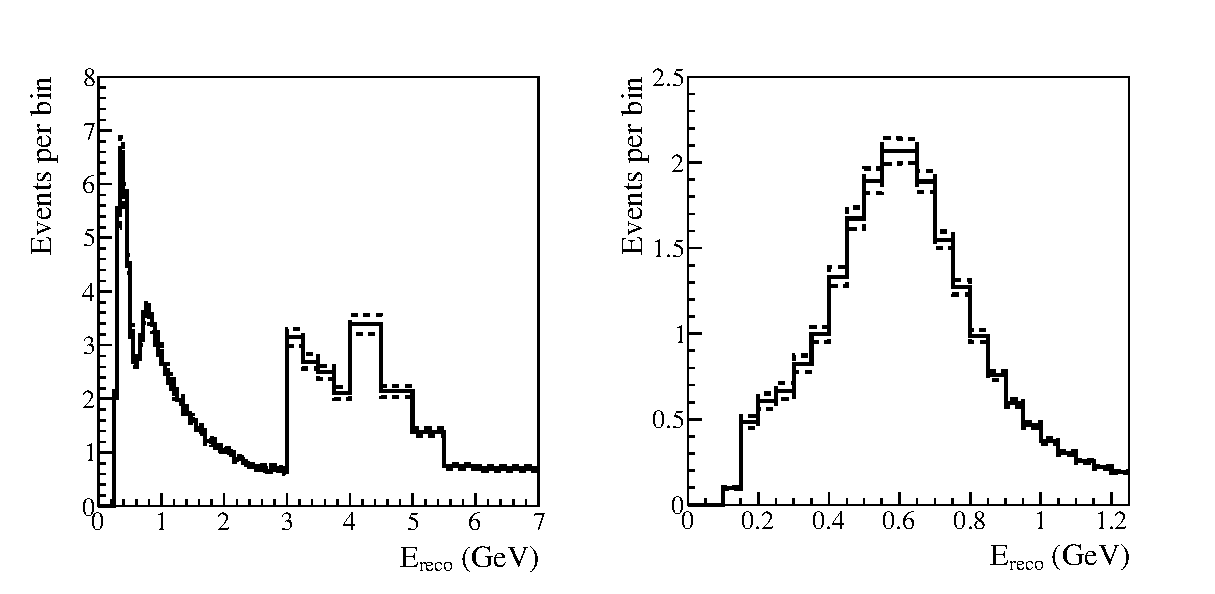
\includegraphics[width=30pc]{./images/systematics/Error_envelope_BANFF.eps}
\caption {
  Error envelope of the single $\mu$-like ring and single e-like event reconstructed energy spectra,
  for oscillations with typical values and the normal mass hierarchy assumed, for the BANFF systematic parameters.
  The numbers shown were calculated for an exposure of 6.5700$\times$10$^{20}$ POT.
  BANFF-tuned MC templates were used.
  The error envelope was calculated as the $\pm$1$\sigma$ spread of bin contents using an ensemble of 20k toy MC experiments generated with randomized BANFF systematic parameters, taking into account their correlations.
}
\label{fig:error_envelope_banff}
\end{figure*}


\begin{figure*}[htb]
\center
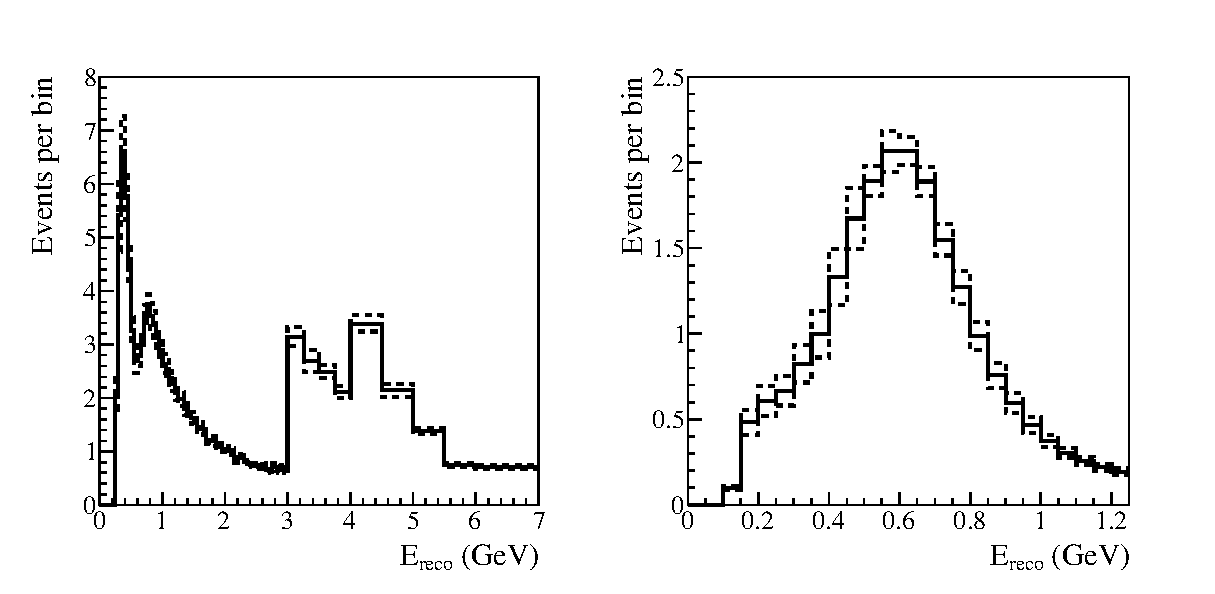
\includegraphics[width=30pc]{./images/systematics/Error_envelope_xsec.eps}
\caption {
  Error envelope of the single $\mu$-like ring and single e-like event reconstructed energy spectra,
  for oscillations with typical values and the normal mass hierarchy assumed, for the uncorrelated cross-section systematic parameters.
  The numbers shown were calculated for an exposure of 6.5700$\times$10$^{20}$ POT.
  BANFF-tuned MC templates were used.
  The error envelope was calculated as the $\pm$1$\sigma$ spread of bin contents using an ensemble of 20k toy MC experiments generated with randomized uncorrelated cross-section systematic parameters.
}
\label{fig:error_envelope_xsec}
\end{figure*}


\begin{figure*}[htb]
\center
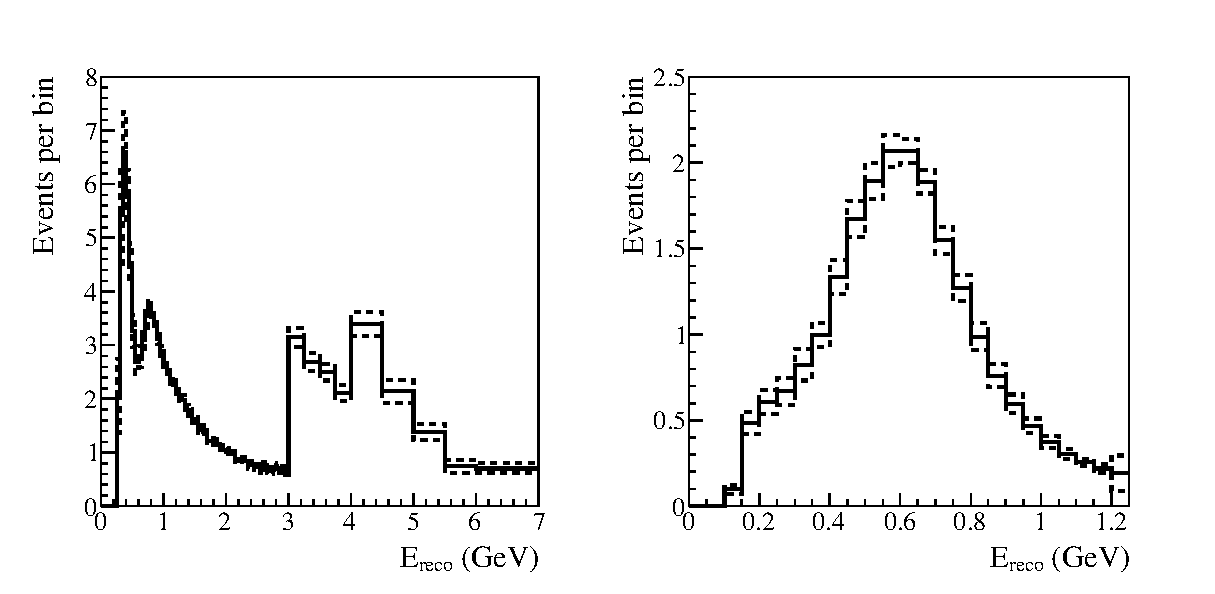
\includegraphics[width=30pc]{./images/systematics/Error_envelope_skfsi_final.eps}
\caption {
  Error envelope of the single $\mu$-like ring and single e-like event reconstructed energy spectra,
  for oscillations with typical values and the normal mass hierarchy assumed, for the SK+FSI systematic parameters.
  The numbers shown were calculated for an exposure of 6.5700$\times$10$^{20}$ POT.
  BANFF-tuned MC templates were used.
  The error envelope was calculated as the $\pm$1$\sigma$ spread of bin contents using an ensemble of 20k toy MC experiments generated with randomized SK+FSI systematic parameters, taking into account their correlations.
}
\label{fig:error_envelope_skfsi}
\end{figure*}

\begin{figure*}[htb]
\center
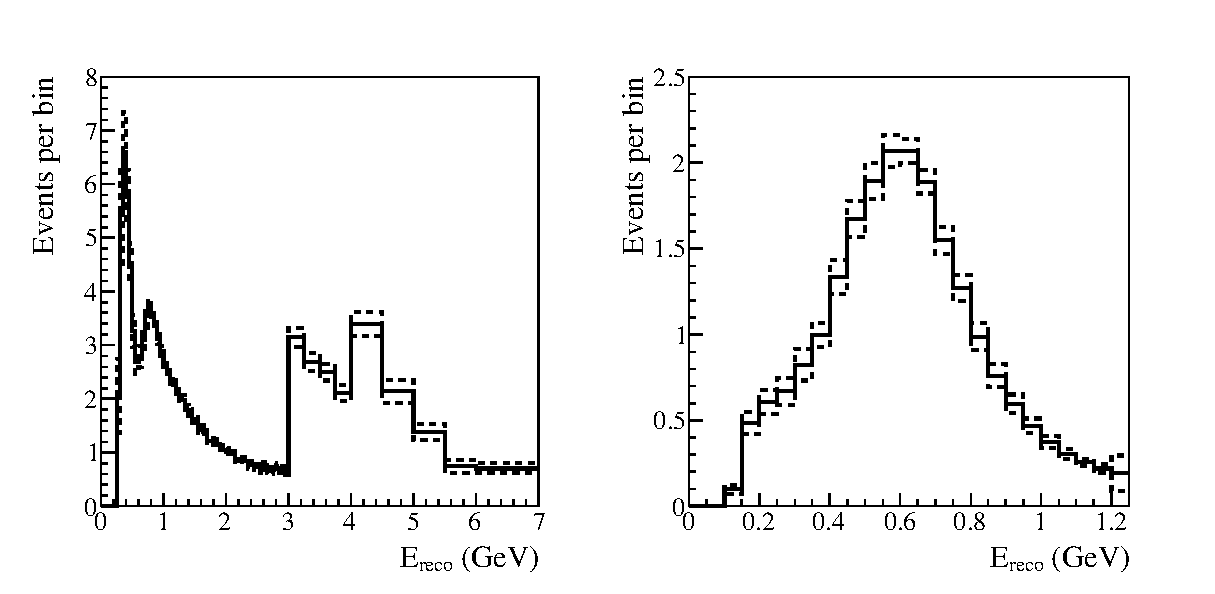
\includegraphics[width=30pc]{./images/systematics/Error_envelope_skfsi_final.eps}
\caption {
  Total error envelope of the single $\mu$-like ring and single e-like event reconstructed energy spectra,
  for oscillations with typical values and the normal mass hierarchy assumed.
  The numbers shown were calculated for an exposure of 6.5700$\times$10$^{20}$ POT.
  BANFF-tuned MC templates were used.
  The error envelope was calculated as the $\pm$1$\sigma$ spread of bin contents using an ensemble of 20k toy MC experiments generated with all systematic parameters randomized, taking into account their correlations.
}
\label{fig:error_envelope_total}
\end{figure*}


\begin{figure*}[htb]
\center
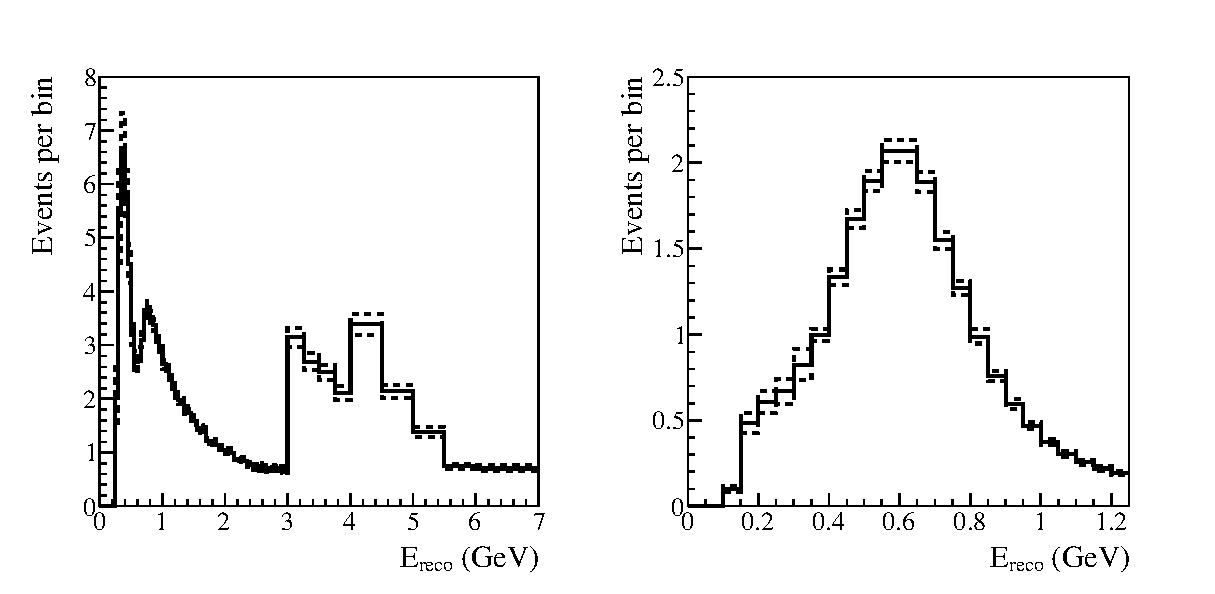
\includegraphics[width=30pc]{./images/systematics/Error_envelope_skfsi_final_noEscale.eps}
\caption {
As in Fig. \ref{fig:error_envelope_skfsi}, but not tweaking the reconstructed energy scale systematic. 
}
\label{fig:error_envelope_skfsi_noEscale}
\end{figure*}



\begin{figure*}[htb]
\center
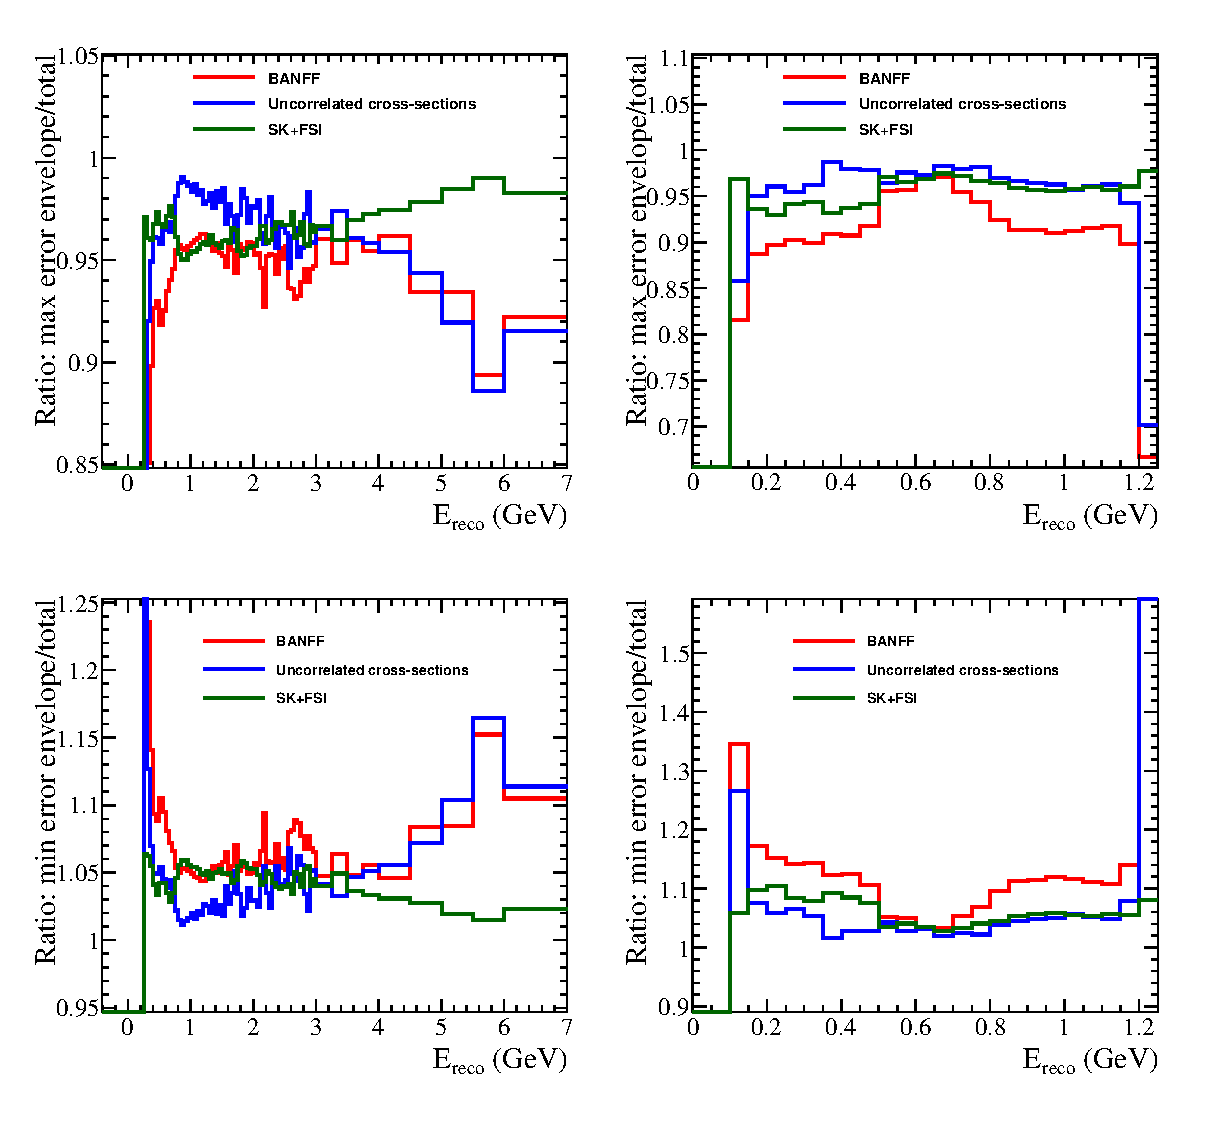
\includegraphics[width=30pc]{./images/systematics/Ratios_error_envelopes.eps}
\caption {
Ratios of the error envelopes in Figs. \ref{fig:error_envelope_banff}-\ref{fig:error_envelope_skfsi} to the total error envelope in Fig. \ref{fig:error_envelope_total} for the maximum (top plots) and minimum (bottom plots) spread.
}
\label{fig:error_envelope_ratios}
\end{figure*}

%..................





